% NOTES:
%%    do we want to explore for larger S?  Does false positive rate change?

% TODO:
%   reference tables!!
%   @put in the missing reference
%   @do we want to partition hchc and metahit?

\documentclass{pnastwo}
\pdfoutput=1
%\documentclass[draft]{pnastwo}
%\usepackage[pdftex]{graphicx}
\usepackage{graphicx}
%\graphicspath{{figures/}}

\begin{document}

\title{Scaling metagenome sequence assembly with probabilistic de Bruijn
graphs}

\author{
Jason Pell
\affil{1}{Computer Science and Engineering, Michigan State University, East Lansing, MI, United States}
\and
Arend Hintze
\affil{1}{}
\and
Rosangela Canino-Koning
\affil{1}{}
\and
Adina Howe
\affil{2}{Microbiology and Molecular Genetics, Michigan State University, East Lansing, MI, United States}
\and
James M. Tiedje
\affil{2}{}
\affil{3}{Crop and Soil Sciences, Michigan State University, East Lansing, MI, United States}
\and
C. Titus Brown
\affil{1}{}
\affil{2}{}
\footnote{Corresponding author: ctb@msu.edu}
}

\maketitle

%{\center
%Classification:\\
%Physical Sciences, Computer Sciences;\\
%Biological Sciences, Biophysics and Computational Biology\\
%}

\begin{article}

\begin{abstract}

The memory requirements for de novo assembly of short-read shotgun
sequencing data from complex microbial populations are an increasingly
large practical barrier to environmental studies.  Here we introduce a
memory-efficient graph representation with which we can analyze the
k-mer connectivity of metagenomic samples, allowing us to reduce the
size of the de novo assembly process for metagenomes with a partitioning 
step to divide the assembly graph into separate groups. This graph 
representation is based on a
probabilistic data structure, a Bloom filter, that allows us to store
assembly graphs in as little as 4 bits per k-mer.  We use this
approach to achieve a nearly 40-fold decrease in memory for the assembly of a
soil metagenome sample.

\end{abstract}

\keywords{metagenomics | de novo assembly | de Bruijn graphs | k-mers}

\section{Introduction}



De novo assembly of shotgun sequencing reads into longer contiguous
sequences plays an important role in virtually all genomic research
\cite{pubmed19482960}.
However, current computational methods for sequence assembly do not
scale well to the volume of sequencing data now readily available from
next-generation sequencing machines \cite{pubmed19482960,pubmed22147368}.  In particular, the deep
sequencing required to sample complex microbial environments easily
results in data sets that surpass the working memory of available
computers \cite{metahit,rumen}.

Shotgun sequencing produces hundreds of millions or billions of short
sequences that are randomly read from the sample, and assembly of
these short sequences into longer, non-redundant sequences is
critically important for gene content analysis \cite{pubmed19482960}.  The process of
sequence assembly relies upon connecting many short
sequences, and efficient connectivity analysis in turn requires a
substantial amount of working memory in order to store overlaps,
which limits many assemblers \cite{pubmed22147368}.

Assembly of these short reads is particularly important for the sequencing
and analysis of complex microbial ecosystems, which can contain
thousands and even millions of different microbial species \cite{pubmed20195499,pubmed16123304}.  These
ecosystems mediate important biogeochemical processes but are still
poorly understood at a molecular level, in large part because they
consist of many microbes that cannot be cultured or studied
individually in the lab \cite{pubmed20195499}.  Ensemble sequencing (``metagenomics'') of
these complex environments is one of the few ways to render them
accessible, and has resulted in substantial early progress in
understanding the microbial composition and function of the ocean, human gut, cow
rumen, and permafrost soil \cite{metahit,rumen,sargasso,permafrost}.  However, as sequencing capacity grows,
the assembly of sequences from these complex samples has become
increasingly computationally challenging.  Current methods for short-read assembly rely on
inexact data reduction in which reads from low-abundance organisms are
discarded, biasing analyses towards high-abundance organisms \cite{metahit,rumen,permafrost}.

The predominant assembly formalism applied to short-read sequencing
data sets is a de Bruijn graph \cite{pubmed11504945,pubmed20211242,pubmed22068540}.
In a de Bruijn graph approach, sequencing reads are decomposed into
fixed-length words, or k-mers, and used to build a connectivity graph.
This graph is then traversed to determine contiguous sequences
\cite{pubmed22068540}.  Because de Bruijn graphs store only k-mers,
memory usage scales with the number of unique k-mers in the data set
rather than the number of reads.  Thus human genomes can be assembled
with less than 512GB of system memory \cite{pmid21187386}.  For more
complex samples such as soil metagenomes, which may possess millions
or more species, terabytes of memory would be required to store the graph.  Moreover, the wide variation in species abundance
limits the utility of standard memory-reduction practices such as
abundance-based error-correction \cite{pubmed21114842}.

In this work, we describe a simple probabilistic representation for
storing de Bruijn graphs in memory, based on Bloom filters
\cite{bloom}.  Bloom filters are fixed-memory probabilistic data
structures for storing sparse sets; essentially hash tables without collision
detection, set membership queries on Bloom filters can yield false
positives -- elements marked as present that do not actually exist --
but not false negatives. While Bloom filters have been used in Bioinformatics 
software tools in the 
past\cite{bloomref1,bloomref2,bloomref3,bloomref4}, to our knowledge this is 
the first time they have been used for assembly graph traversal. We show that 
this probabilistic graph
representation can be used to efficiently store and traverse DNA de
Bruijn graphs with 20 to 40-fold decrease in memory usage
over two common de Bruijn graph-based assemblers, Velvet
and ABySS~\cite{velvet,abyss}. We relate 
changes in local and
global graph connectivity to the false positive rate of the underlying
Bloom filters, and show that the graph's global structure is accurate
for false positive rates of 15\% or lower, 
corresponding to a lower memory limit of approximately
4 bits per graph node.

We apply this graph representation to reduce the memory needed
to assemble a soil metagenome sample, through
the use of read partitioning.  Partitioning separates a de Bruijn graph up
into disconnected graph components; these components can be used to
subdivide sequencing reads into disconnected subsets that can be
assembled separately.
This exploits a convenient biological
feature of metagenomic samples: they contain many microbes that should
not assemble together.  Graph partitioning has
been used to improve the quality of metagenome and transcriptome assemblies
by adapting assembly parameters to local coverage of the graph~\cite{metavelvet,pubmed21685107,trinity}.  However, to our knowledge, partitioning has not been applied
to scaling metagenome assembly. By applying the
probabilistic de Bruijn graph representation to the problem of
partitioning, we achieve a dramatic decrease of nearly 40-fold in the memory
required for assembly of a soil metagenome.

% @@ exact/inexact data influence

\section{Results}

\subsection{Bloom filters can store de Bruijn graphs}

Given a set of short DNA sequences, or reads, we first break down each
read into a set of overlapping k-mers.  We then store each k-mer in a
Bloom filter, a probabilistic data structure for storing elements from sparse data
sets (see \emph{Methods} for implementation details).  Each k-mer
serves as a vertex in a graph, with an edge between two vertices $N_1$
and $N_2$ if and only if $N_1$ and $N_2$ share a (k-1)-mer that is a
prefix of $N_1$ and a postfix of $N_2$, or vice versa (see Figure
\ref{fig:bloomgraph}).  This edge is not stored explicitly.

Thus each k-mer has up to 8 edges connecting to 8 neighboring k-mers, which can be determined by
simply building all possible 1-base extensions and testing for their
presence in the Bloom filter.  In doing so, we implicitly treat the
graph as a simple graph as opposed to a multigraph, which
means that there can be no self-loops or parallel edges between
vertices/k-mers.  By relying on Bloom filters, the size of the data structure 
is fixed: no extra memory is used as additional data is
added.

This graph structure is effectively {\em compressible} because one can
choose a larger or smaller size for the underlying Bloom filters; for
a fixed number of entries, a larger Bloom filter has lower occupancy
and produces correspondingly fewer false positives, while a smaller
Bloom filter has higher occupancy and produces more false
positives. In exchange for memory, we can store k-mer nodes more or
less accurately: for example, for a false positive rate of 15\%, at
which 1 in 6 random k-mers tested would be falsely considered present,
each real k-mer can be stored in under 4 bits of memory (see
Table~\ref{table:bitskmer}).	

Using a probabilistic data structure to store k-mer nodes does
cause one potential problem: in contrast to an exact graph storage, there is a chance that a k-mer
will be adjacent to a false positive k-mer.  That is, a k-mer may
connect to another k-mer that does not actually exist in the original
dataset but nonetheless registers as present, due to the probabilistic
nature of the Bloom filter.  As the memory per real k-mer is
decreased, false positive vertices and edges are gained, so
compressing the graph results in a more tightly interconnected graph.
If the false positive rate is too high, the graph structure will be
dominated by false connectivity -- but what rate is ``too high''?  We
study this key question in detail below.

\subsection{False positives cause local elaboration of graph structure}

Erroneous neighbors created by false positives can alter the graph
structure.  To better understand this effect, we generated a random
1,031bp circular sequence and visualized the effect of different false
positive rates.  After storing this single sequence in compressible
graphs using $k=31$ with four different false positive rates
($p_f$=0.01, 0.05, 0.10, and 0.15), we explored the graph using
breadth-first search beginning at the first 31-mer.  The graphs in
Figure \ref{fig:circles} illustrate how the local graph structure elaborates with the
false positive rate while the overall circular graph structure
remains, with no erroneous shortcuts between k-mers that are present
in the original sequence.  It is visually apparent that even a high false positive rate of 15\% does not systematically and erroneously connect distant k-mers.

In addition, it is simple to see that a linear increase in the false 
positive rate results in a linear increase in the number of expected 
neighbors for a particular k-mer. For most isolated k-mers (i.e. no adjacent 
``real'' k-mers), the calculation is 
E(erroneous neighbors)$ = 8 \times p_f$. Thus, the local graph 
structure breaks down in a linear fashion.  Does the global graph structure
degrade in a similar fashion?

\subsection{False long-range connectivity is a nonlinear function of the false positive rate}

To explore the point at which our data structure systematically
engenders false long-range connections, we inserted random k-mers
into Bloom filters with increasing false positive rates.  These k-mers
connect to other k-mers to form graph components that increase
in size with the false positive rate.
We then
calculated the average component size in the graph for each false positive rate
($n=10000$) and used percentile bootstrap to obtain estimates within a
95\% confidence interval. Figure \ref{fig:clustersize} demonstrates that the average component size
rapidly increases as a specific threshold is approached, which appears
to be at a false positive rate near 0.18 for k=31. Beyond 0.18, the components
begin to join together into larger components.

As the false positive rate increases, we observe a sudden transition
from many small components to fewer, larger components created by erroneous connections between the ``true'' components (Figure \ref{fig:clustersize}).  In contrast to the linear increase in the
local neighborhood structure as the false positive rate increases
linearly, the change in global graph structure is abrupt as previously
disconnected components join together.  This rapid change resembles a
geometric phase transition, which for graphs can be discussed in terms of
percolation theory~\cite{staufferintro}. We can map our problem to site percolation by
considering a probability $p$ that a particular k-mer is present, or ``on''. (This is in contrast to bond percolation where $p$ represents
the probability of a particular edge being present.) As
long as the false positive rate is below the percolation threshold
$p_\theta$ (i.e. in the subcritical phase), we would predict that the graph
is not highly connected by false positives.

% @CTB MENTION ITERATIVE PARTITIONING

Percolation thresholds for finite graphs can be estimated by finding
where the component size distribution transitions from linear to
quadratic in form \cite{stauffer1979scaling}.  Using the calculation
method described in \emph{Methods}, we found the site percolation
threshold for DNA de Bruijn graphs to be $p_\theta = 0.183 \pm 0.001$
for k between 5 and 12.
Although we only tested within this limited range of k, the
percolation threshold appears to be independent of different $k$ (see
Figure~S1).
Thus, as long as the false positive rate is below $0.183$, we
predict that truly disconnected components in the graph are unlikely
to connect to one another erroneously, that is, due to errors
introduced by the probabilistic representation.

\subsection{Large-scale graph structure is retained up to the percolation threshold}

The results from component size analysis and the percolation threshold
estimation suggest that global connectivity of the graph is unlikely
to change below a false positive rate of 18\%.  Do we see this invariance
in global connectivity in other graph measures?

To assess global connectivity, we employed the diameter metric in
graph theory, the length of the ``longest shortest'' path between any two
vertices~\cite{bondy2008graph}.  If shorter paths were being systematically
generated due to false positives, we would expect the diameter of components to
decrease as the false positive rate increased.
We randomly generated 58bp
long circular chromosomes (50bp read with the first 8-mer appended to the 
end of the string) to construct components containing 50 8-mers
and calculated the diameter at different false positive rates. We kept 
$k$ low because we needed to be able to exhaustively explore the graph 
even beyond the percolation threshold, which is computationally 
prohibitive to do at higher k values. Furthermore, larger circular chromosomes 
would be more likely to erroneously connect at a fixed $k$, but due to the 
relatively low number of possible 8-mers, we had to keep the chromosomes 
small.  
We only considered paths
between two real k-mers in the dataset.  
At each
false positive rate, we ran the simulation 500 times and estimated the
mean within a 95\% confidence interval using percentile bootstrap. As
Figure~\ref{fig:diam} shows, erroneous connections between pairs of
real k-mers are rare below a false positive rate of 20\%.
For false positive rates above this threshold, spurious
connections between real k-mers are created, which lowers the
diameter.  Thus, the larger scale graph structure is retained up through
$p = 0.183$, as suggested by the component size analysis and
percolation results.

\subsection{Erroneous k-mers from sequencing eclipse graph false positives}

It is important to compare the errors from false positives in the de
Bruijn graph representation with errors from real data.  In particular,
real data from massively parallel sequencers will contain base
calling errors.  In de Bruijn graph-based assemblers, these sequencing
errors add to the graph complexity and make it more difficult to find
high-quality paths for generating long, accurate contigs. Since our
approach also generates false positives, we wanted to compare the
error rate from the Bloom filter graph with experimental errors
generated by sequencing (Table \ref{table:ecoli}). We used the \emph{E. coli} K-12
MG1665 genome to compare various graph invariants between an Illumina
dataset generated from the same strain (see \emph{Methods}), an exact
representation of the genome, and inexact representations with
different false positive rates.

For these comparisons, we used a $k$ value of 17, which allows us to
use enough a bitmap for exact graph storage, i.e. we have no
false positives because we can store $4^{17}$ entries precisely in
2GB of system memory. This is equivalent to a Bloom filter with one 
hash table and a 0\% false positive rate.
We found a
total of 50,605 17-mers in the exact representation that were not part
of a simple line, i.e. had more than two neighbors (degree $>$ 2). As
the false positive rate increased, the number of these 17-mers
increased in the expected linear fashion.
% in addition to the number of
%false positive 17-mers found in each component.
Furthermore, the
number of real 17-mers, those that are not false positives,
comprise the majority of the graph.

In contrast, when we examined an exact representation of an Illumina
dataset, only 9.9\% of the k-mers in the graph truly exist in the
reference genome.  As above, we only counted false positive k-mers
that are transitively connected to least one real k-mer. The number of
17-mers with more than 2 neighbors is higher than for the exact
representation of the genome, which demonstrates that sequencing
errors add to the complexity of the graph. Overall, the
errors demonstrated by sequencers dwarf the errors caused by the
inexact graph representation below a reasonable false positive rate.

When we assemble this data set with the Velvet and ABySS assemblers at
k=31, Velvet requires 3.7GB to assemble the data set,
while ABySS requires 1.6GB; this memory usage is dominated by the
graph storage \cite{zerbinothesis}. Thus the Bloom filter approach stores graphs 30 or
more times more efficiently than either program, even with a low false
positive rate of 1\%.  While this direct comparison can not be made fairly -- assemblers store the graph as well as k-mer abundances and other information -- it does suggest that there are opportunities for improving memory usage.

\subsection{Sequences can be accurately partitioned by graph connectivity}


Can we use this low-memory graph representation to find and separate
components in de Bruijn graphs?  The primary concern is that false positive
nodes or edges would connect components, but the diameter results suggest that
components are unlikely to connect below a 20\% false positive rate.
To verify this, we analyzed a simulated dataset of 1,000
randomly generated sequences of length 10,000 bp.  Using $k=31$,
we partitioned the data across many different false positive rates,
using the procedure described in \emph{Methods}. As predicted, the
resulting number of partitions did not vary across the false positive
rates while $f_p \le 0.15$ (Figure \ref{fig:partfp}).

We then applied partitioning to a considerably larger bulk soil
metagenome (``MSB2'') containing 35 million 75 bp long reads generated
from an Illumina GAII sequencer.  We calculated the number of unique
31-mers present in the data set to be 1.35 billion. Then, for each of
several false positive rates (see Table \ref{table:parts}) we loaded
the reads into a graph, eliminated components containing fewer than
200 unique k-mers, and partitioned the reads into separate files based
on graph connectivity.

Once we obtained the partition sets, we individually assembled each
set of partitions using ABySS, as well as the entire (unpartitioned) 
data set,
retaining contigs longer than 500 bp.  The resulting assemblies were
all identical, containing 1,444 contigs with a total assembled
sequence of 1.07 megabases.  The unpartitioned data set required 33GB to
assemble with ABySS, while the partitioned data sets all required
under 1.75GB to partition into seperate components and assemble -- 
a decrease in over 18x
in memory usage for an identical result.

% @CTB repartitioning

\section{Discussion}

% @@ reorder so concluding thoughts come up top? naah.

\subsection{Bloom filters can be used to efficiently store de Bruijn graphs}

The use of Bloom filters to store a de Bruijn graph is
straightforward and memory efficient.  The expected false positive
rate can be tuned based on desired memory usage,
yielding a wide range of possible storage efficiencies
(Table \ref{table:bitskmer}). Since memory usage is k independent 
in Bloom filters, it is more efficient than the theoretical lower-bound 
for a lossless exact representation when the number of k-mers inserted 
in the graph is sparsely populated, which is dependent on k (Figure~S2).

Even for low false positive rates such as 1\%, this is still an
efficient graph representation, with a greater than 30-fold
improvement in memory usage over two existing assemblers, Velvet and
ABySS (Table \ref{table:ecoli}).  We can store k-mers in this data structure with a much smaller
set of ``erroneous'' k-mers than those generated by sequencing errors,
and the Bloom filter false positive rates have less of an effect on
branching graph structure than do sequencing errors.  In addition, the
false positives engendered by the Bloom filters are uncorrelated with
the original sequence, unlike single-base sequencing errors which resemble
the real sequence.  This feature may further
reduce the effect of false positives on de Bruijn graph analysis,
depending on the specific application.

\subsection{Preservation of long-range structure permits graph partitioning}

Using a probabilistic graph representation with false positive nodes
and edges raises the specter of systematic graph artifacts resulting
from the false positives.  For partitioning, the primary concern is that false
positives will incorrectly connect components, rendering partitioning
ineffective.  Our results from percolation analysis, diameter
calculations, and partitioning of simulated and real data demonstrate that
below the calculated percolation threshold this is not a significant
problem.  As long as the false positive rate is below 18.3\%,
long false paths are not spontaneously created and the
large scale graph properties do not change.  Above this rate, the global
graph structure slowly degrades.

Our partitioning results on a real soil metagenome, the MSB2 data set,
demonstrate the utility of partitioning for reducing memory usage.
For this specific data set, we obtained {\em identical} results with a
20-40x decrease in memory (Table \ref{table:parts}).  This is consonant with our results from
storing the E. coli genome, in which we achieved a 30-fold decrease
in memory usage over the exact representation at a false positive rate
of 1\%.  While increased coverage and variation in data set complexity
will affect actual memory usage for other data sets, these results demonstrate that
significant scaling in the memory required for assembly can be achieved
in at least one real case.

The memory requirements for the partitioning process on the MSB2 data
set are dominated by the memory required to store and explore the
graph; the higher memory usage observed for partitioning at a false positive rate
of 15\% is due to the increase in component size from local false
positives.  Regardless, the memory requirements for downstream assembly
of partitions is driven by the size of the largest partition, which
here is very small (345,000 reads; Table \ref{table:parts}) due to the
high diversity of soil and the concordant low coverage.  The
dominant partition size is remarkably refractory to the graph's false
positive rate, increasing by far less than 1\% for a 15-fold increase
in false positives; this shows that our theoretical and
simulated results for component size and diameter apply to the MSB2 data set
as well.

% @CTB fill in number

There are several biological problems that are particularly well
suited to a partitioning approach.  Like metagenomes, transcriptomes
consist of populations of many {\em disconnected} sequences.  This has
already been exploited for assembly improvement: Trinity relies on a
partitioning approach in the second phase of transcriptome assembly;
and both Meta-IDBA and MetaVelvet rely on locality of coverage and and
discovery of components for metagenome assembly
\cite{metavelvet,pubmed21685107,trinity}.  Once partitioned, components
can be assembled with parameters chosen for the coverage and sequence
heterogeneity present in each partition.  Moreover, data sets partitioned
at a low $k_0$ can be exactly assembled with any $k \ge k_0$, because
overlaps of $k_0-1$ bases include all overlaps of greater length.
Existing approaches to partitioning, however,
rely on exact graph representations that are significantly more memory intensive
than the one presented here.  The utility of the probabilistic graph
representation for partitioning rests on its significantly lower
memory usage.

Combined with the scaling
properties of the graph representation, partitioning with this probabilistic
de Bruijn graph representation offers a way to
efficiently apply a partitioning strategy to certain
assembly problems.  While this work focuses on theoretical properties
of the graph representation, the next step will be to evaluate the approach
on many real data sets.

\subsection{Concluding thoughts}

% @@ read, cite references from pop

Developing efficient and accurate approaches to de novo assembly
continues to be one of the ``grand challenges'' of bioinformatics
\cite{pubmed22147368}.  Improved metagenome assembly approaches are
particularly important for the investigation of microbial life on Earth, much
of which has not been sampled \cite{terabasemetag}.  While our appreciation
for the role that microbes play in biogeochemical processes is
only growing ,
we are increasingly limited by our ability to analyze the data.  For
example, the Earth Microbiome Project is generating petabytes of
sequencing data from complex microbial communities, many of which
contain entirely novel ensembles of microbes; scaling de novo assembly
is a critical part of this investigation \cite{emp2010}.

The probabilistic de Bruijn graph representation presented here has a
number of convenient features for storing and analyzing large assembly
graphs.  First, it is efficient and compressible: for a given data
set, a wide range of false positive rates can be chosen without
impacting the global structure of the graph, allowing graph storage in
as little as 4 bits per k-mer.  Because a higher false positive rate
yields a more elaborate local structure, memory can be traded for
traversal time in e.g. partitioning.  Second, it is a fixed-memory
data structure, with predictable degradation of both local and global
structure as more data is inserted.  For data sets where the number of
unique k-mers is not known in advance, the occupancy of the Bloom
filter can be monitored as data is inserted and directly converted
to an expected false positive rate.  Third, the memory usage is
independent of the k-mer size chosen, making this representation
convenient for exploring properties at many different parameters.  It
also allows the storage and traversal of de Bruijn graphs at multiple
k-mer sizes within a single structure, although we have not yet
explored these properties.  And fourth, it supports memory-efficient
partitioning, a ``divide-and-conquer'' approach that exploits underlying biological features of
the data.

Our initial motivation for developing this use of Bloom filters was to
explore partitioning as an approach to scaling metagenome assembly,
but there are many additional uses beyond metagenomics.  Here we describe
exact partitioning of the graph into components, but {\em inexact}
partitioning has been successfully applied to mRNAseq assembly \cite{trinity}.  Inexact partitioning, as done by the Chrysalis component of the Trinity pipeline, uses heuristics to subdivide the graph for later assembly,
and this data structure should be usable for this purpose as well.
More broadly, a more memory efficient de Bruijn graph representation opens up
many additional opportunities.  While de Bruijn graph approaches are currently
being used primarily for the purposes of assembly, they are a generally
useful formalism for sequence analysis. In particular, they have been
extended to efficient multiple-sequence alignment,
repeat discovery, and detection of local and
structural sequence variation \cite{zerbinothesis,zhang2003dna,price2005novo,iqbalcortex}.  We are also
exploring the use of de Bruijn graphs for graph-based homology search
and artifact detection in large sequencing data sets.  The ability to
more efficiently store graphs in memory may also result in
additional uses for de Bruijn graphs.

\begin{materials}

\section{Genome and Sequence Data}
We used the \emph{E. coli} K-12 MG1655 genome (GenBank: U00096.2) and two MG1655 Illumina 
datasets (Short Read Archive accessions SRX000429 and SRX000430) for E. coli
analyses.  The MSB2 soil data set is available as SRA accession SRA050710.1.

\section{Data Structure Implementation}
We implemented a variation on the Bloom filter data structure to store
k-mers in memory. In a classic Bloom filter, multiple hash functions
map bits into a single hash table to add an object or test for the presence
of an object in the set. In our variant, we use multiple
prime-number-sized hash tables, each with a different hash
function corresponding to the modulus of the DNA bitstring
representation with the hash table size; this is a computationally convenient way to construct hash functions for DNA strings.  The underlying properties of
the Bloom filter are identical.  To add a k-mer to the
filter, the corresponding bit in each hash table is set to 1.  To find
a k-mer, each table is queried for the presence of
that k-mer; for a k-mer to be considered present in the dataset, the
k-mer must be found in all of the hash tables.  If a k-mer is not
present in any one hash table, then it is certainly not in the
dataset. This explains the one-sided error: false positives are
possible but false negatives are not. The expected false positive rate
is simply the product of the occupancies of the hash tables.  As with
other hash-style data structures, Bloom filters have a fast lookup
time, $O(h)$ for $h$ hash tables.  Similar to other hash-style data
structures for storing k-mers, memory usage is independent of the
value of $k$.

\section{Calculating Data Structure Properties}
The properties of our Bloom filter variant are the
same as a classical Bloom filter \cite{bloomsurvey}.
To calculate the expected false positive 
rate, we
take the product of the occupancy of each hash table:
\begin{displaymath}
P_f = \prod_{h \in H} occ(h)
\end{displaymath}
where $h$ is a hash table in the set of hash tables $H$ and $occ$ denotes
the occupancy (proportion of bits set) for a hash table.
We find the optimal number of hash tables
to use by calculating
\begin{displaymath}
\vert H \vert_{opt} = \ln 2 \frac{m}{k}
\end{displaymath}
where $m$ is the amount of memory in bits to allocate and $k$
is the number of unique k-mers to be inserted. Finally,
the number of bits per
k-mer used in the data structure for the optimal number of hash 
tables is

\begin{displaymath}
\frac{m}{n} = \frac{1}{\ln(2)} \log{\frac{1}{P_f}}.
\end{displaymath}

\section{Estimating False Positive Rate For Erroneous Connectivity}
We ran a simulation to find when components in the graph 
begin to erroneously connect to one another.
To calculate the false positive rate $p$ at which this aberrant 
connectivity occurs, 
we added random k-mers, sampled from a uniform GC distribution, to the data structure 
and then calculated the occupancy and size of 
the largest 
component. From this we sampled the relative size of 
the largest component and the overall component size distribution for each
given occupancy rate.
At the occupancy where a ``giant component'' appears, this component size distribution 
should be scale-free \cite{stauffer1979scaling}. 

We then found at what value of $p$ the resulting 
component size distribution in logarithmic 
scale can be better fitted in a linear or quadratic fashion using 
the F-statistic
\newline
\newline
\begin{displaymath}
F=\frac{RSS_1-RSS_2}{p_2-p_1} \times \frac{n - p_2}{RSS_2}
\end{displaymath}

where $RSS_i$ is the residual sum of squares for model $i$, $p_i$ is 
the number of parameters for model $i$, and $n$ is the number of data 
points. To handle the finite size sampling error, the data was binned using the 
threshold binning method \cite{adami2002critical}. The critical value for 
when aberrant connectivity occurred was found by determining the local maxima 
of the F-values \cite{wald43}.

\section{Graph Partitioning Using A Bloom Filter}

We used the Bloom filter data structure containing the k-mers from a
dataset to discover components of the graph, i.e. to partition the
graph.  Here a component is a set of k-mers whose originating reads
overlap transitively by at least $k-1$ base pairs.  Reads belonging only
to small components can be discovered and eliminated in fixed
memory using a simple traversal algorithm that truncates after
discovering more than a given number of novel k-mers.  For discovering
large components we tag the graph at a minimum density by using the
underlying reads as a guide.  We then exhaustively explore the graph
around these tags in order to connect tagged k-mers based on graph
connectivity.  The underlying reads in each component can then be
separated based on their partition.

\section{Assembler software}

We used ABySS v1.3.1 and Velvet v1.1.07 to perform assemblies.
The ABySS command was: {\tt mpirun -np 8 ABYSS-P -k31 -o contigs.fa reads.fa}.
The Velvet commands were: {\tt velveth assem 31 -fasta -short reads.fa \&\& velvetg assem}.
We did not use Velvet for the partitioning analysis because Velvet's
error correction algorithm is stochastic and results in dissimilar
assemblies for different read order.

\section{Software and Software Availability}

We have implemented this compressible graph representation and the associated
partitioning algorithm in a
software package named khmer.  It is written in C++ and Python 2.6 and
is available under the BSD open source license at
https://github.com/ctb/khmer.  The graphviz software package was used
for graph visualizations. The scripts to generate the figures of this
paper are available in the khmer repository.

\end{materials}

\begin{acknowledgments}

We thank Chris Adami, Qingpeng Zhang, and Tracy Teal for
thoughtful comments, and Jim Cole and Jordan Fish for discussion of future
applications.  This project was supported by AFRI Competitive Grant
no. 2010-65205-20361 from the USDA NIFA and NSF IOS-0923812, both to CTB.  The
MSB2 soil metagenome was sequenced by the DOE's Joint Genome
Institute through the Great Lakes Bioenergy Research Center.

% @@ also acknowledge adina

\end{acknowledgments}

% @@CTB mention k_0 > k_1 etc.

%\bibliographystyle{abbrv}

%\bibliography{foo2}

\begin{thebibliography}{10}

%\bibitem{nrcbook} National Research Council (US). Committee on Metagenomics 
%and Functional Applications (2007) The new science of metagenomics: revealing 
%the secrets of our microbial planet. {\it Natl Academy Pr}.

\bibitem{pubmed19482960} Pop~M. (2009) Genome assembly reborn: recent 
computational challenges. {\it Brief Bioinform}, 10(4):354--66.

\bibitem{pubmed22147368} Salzberg~S, et al. (2011) GAGE: A critical 
evaluation of genome assemblies and assembly algorithms. {\it Genome Res} 
22(3):557-67.

\bibitem{metahit} Qin ~J, et al. (2010) A human gut microbial gene catalogue 
established by metagenomic sequencing. {\it Nature} \emph{464}, 59--65.

\bibitem{rumen} Hess~M, et al. (2011) Metagenomic discovery of 
biomass-degrading genes and genomes from cow rumen. {\it Science} 
\emph{331}, 463--7.

\bibitem{pubmed20195499} Wooley~J, Godzik~A, and Friedberg~I. (2010) A primer 
on metagenomics. {\it PLoS Comput Biol}, 6(2):e1000667.

\bibitem{pubmed16123304} Gans~J, Wolinsky~M, and Dunbar~J. (2005) 
Computational improvements reveal great bacterial diversity and high metal 
toxicity in soil. {\it Science}, 309(5739):1387--90.

\bibitem{sargasso} Venter~J, et al. (2004) Environmental genome shotgun 
sequencing of the Sargasso Sea. {\it Science} \emph{304}, 66--74.

\bibitem{permafrost} Mackelprang~R, et al. (2011) Metagenomic analysis of a 
permafrost microbial community reveals a rapid response to thaw. {\it Nature}, 
480(7377):368--71.

\bibitem{pubmed11504945} Pevzner~P, Tang~H, and Waterman~M. (2001) An 
Eulerian path approach to DNA fragment assembly. {\it Proc Natl Acad Sci USA},
 98(17):9748--53.

\bibitem{pubmed20211242} Miller~J, Koren~S, and Sutton~G. (2010) Assembly 
algorithms for next-generation sequencing data. {\it Genomics}, 95(6):315--27.

\bibitem{pubmed22068540} Compeau~P, Pevzner~P, and Tesler~G. (2011) How to 
apply de {B}ruijn graphs to genome assembly. {\it Nat Biotechnol}, 
29(11):987--91.

\bibitem{pmid21187386} Gnerre~S, et al. (2011) High-quality draft assemblies 
of mammalian genomes from massively parallel sequence data. {\it Proc Natl 
Acad Sci USA}, 108:1513--1518.

\bibitem{pubmed21114842} Kelley~D, Schatz~M, and Salzberg~S. (2010) Quake: 
quality-aware detection and correction of sequencing errors. {\it Genome 
Biol}, 11(11):R116.

\bibitem{bloom} Bloom~B. (1970) Space/time tradeoffs in hash coding with 
allowable errors. {\it CACM}, 13(7):422--426.

\bibitem{bloomref1} Shi H. (2010) A parallel algorithm for error correction 
in high-throughput short-read data on CUDA-enabled graphics hardware. {\it 
J Comput Biol}, 17(4):603-615.

\bibitem{bloomref2} Stranneheim~H. (2010) Classification of DNA sequences 
using Bloom filters. {\it Bioinformatics} 26(13):1595-1600.

\bibitem{bloomref3} Malsted~P. (2011) Efficient counting of k-mers in DNA 
sequences using a bloom filter. {\it BMC Bioinformatics} 12:333.

\bibitem{bloomref4} Liu~Y. DecGPU: distributed error correction on 
massively parallel graphics processing units using CUDA and MPI. {\it 
BMC Bioinformatics} 12:85.

\bibitem{velvet} Zerbino~DR, Birney~E. (2008) Velvet: algorithms for de novo 
short read assembly using de Bruijn graphs. {\it Genome Res}, 18(5):821-9.

\bibitem{abyss} Simpson~JT, et al. (2009) ABySS: a parallel assembler for 
short read sequence data. {\it Genome Res}, 19(6):1117-23.

\bibitem{metavelvet} Namiki~T, Hachiya~T, Tanaka~H, and Sakakibara~Y. (2011) 
MetaVelvet: An extension of Velvet assembler to de novo metagenome assembly 
from short sequence reads. {\it ACM Conference on Bioinformatics, 
Computational Biology and Biomedicine}.

\bibitem{pubmed21685107} Peng~Y, Leung~H, Yiu~S, and Chin~F. (2011) Meta-IDBA: 
a de Novo assembler for metagenomic data. {\it Bioinformatics}, 
27(13):i94--i101.

\bibitem{trinity} Grabherr~M, et al. (2011) Full-length transcriptome assembly 
from RNA-Seq data without a reference genome. {\it Nat Biotechnol}, 
29(7):644-52.

\bibitem{staufferintro} Stauffer~D and Aharony~A. (2010) Introduction to 
Percolation Theory. {\it Taylor and Frances e-Library}.

\bibitem{stauffer1979scaling} Stauffer~D. (1979) Scaling theory of 
percolation clusters. {\it Physics Reports}, 54(1):1--74.

\bibitem{bondy2008graph} Bondy~J and Murty~U. (2008) Graph Theory. {\it 
Graduate Texts in Mathematics}.

\bibitem{zerbinothesis} Zerbino~DR. (2009) Genome assembly and comparison 
using de Bruijn graphs. Ph.D. thesis, University of Cambridge.

\bibitem{terabasemetag} Gilbert~J, et al. (2010) Meeting report: the terabase 
metagenomics workshop and the vision of an earth microbiome project. {\it 
Stand Genomic Sci}, 3(3):243--8.

\bibitem{emp2010} Gilbert~J, et al. (2010) The Earth Microbiome Project: 
Meeting report of the ``1 EMP meeting on sample selection and acquisition'' 
at Argonne National Laboratory October 6 2010. {\it Stand Genomic Sci} 
\emph{3}, 249--53.

\bibitem{zhang2003dna} Zhang~Y and Waterman~M. (2003) DNA Sequence Assembly 
and Multiple Sequence Alignment by an Eulerian Path Approach. In {\it Cold 
Spring Harbor Symposia on Quantitative Biology}, volume~68, pp 205--212. 
Cold Spring Harbor Laboratory Press.

\bibitem{price2005novo} Price~A, Jones~N, and Pevzner~P. (2005) De novo 
identification of repeat families in large genomes. {\it Bioinformatics}, 
21(suppl 1):i351--i358.

\bibitem{bloomsurvey}
Broder~A and Mitzenmacher~M. (2004) Network applications of bloom filters: 
A survey. {\it Internet Mathematics}, 1(4):485--509.

\bibitem{adami2002critical} Adami~C and Chu~J. (2002) Critical and 
near-critical branching processes. {\it Phys Rev E}, 66(1):011907.

\bibitem{wald43} Wald~A. (1943) Tests of statistical hypotheses concerning 
several parameters when the number of observations is large. {\it Transactions 
of the American Mathematical Society}, 54:426--482.

\end{thebibliography}

\end{article}

\begin{figure}
\centering
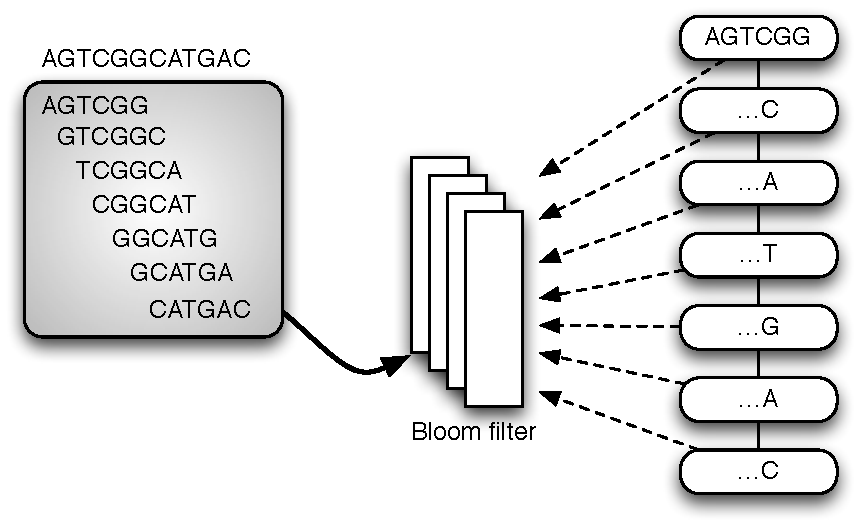
\includegraphics[width=5in]{bloomgraph}
\caption{Storing de Bruijn graphs in Bloom filters.  Longer sequences (top left) are broken down into k-mers (bottom left; here, k=6) and stored in the Bloom filter (middle).
The graph (right) is traversed by starting at a k-mer and then testing all possible 1-base pre- and post-fixes for presence in the Bloom filter.}

\label{fig:bloomgraph}
\end{figure}

\begin{figure}
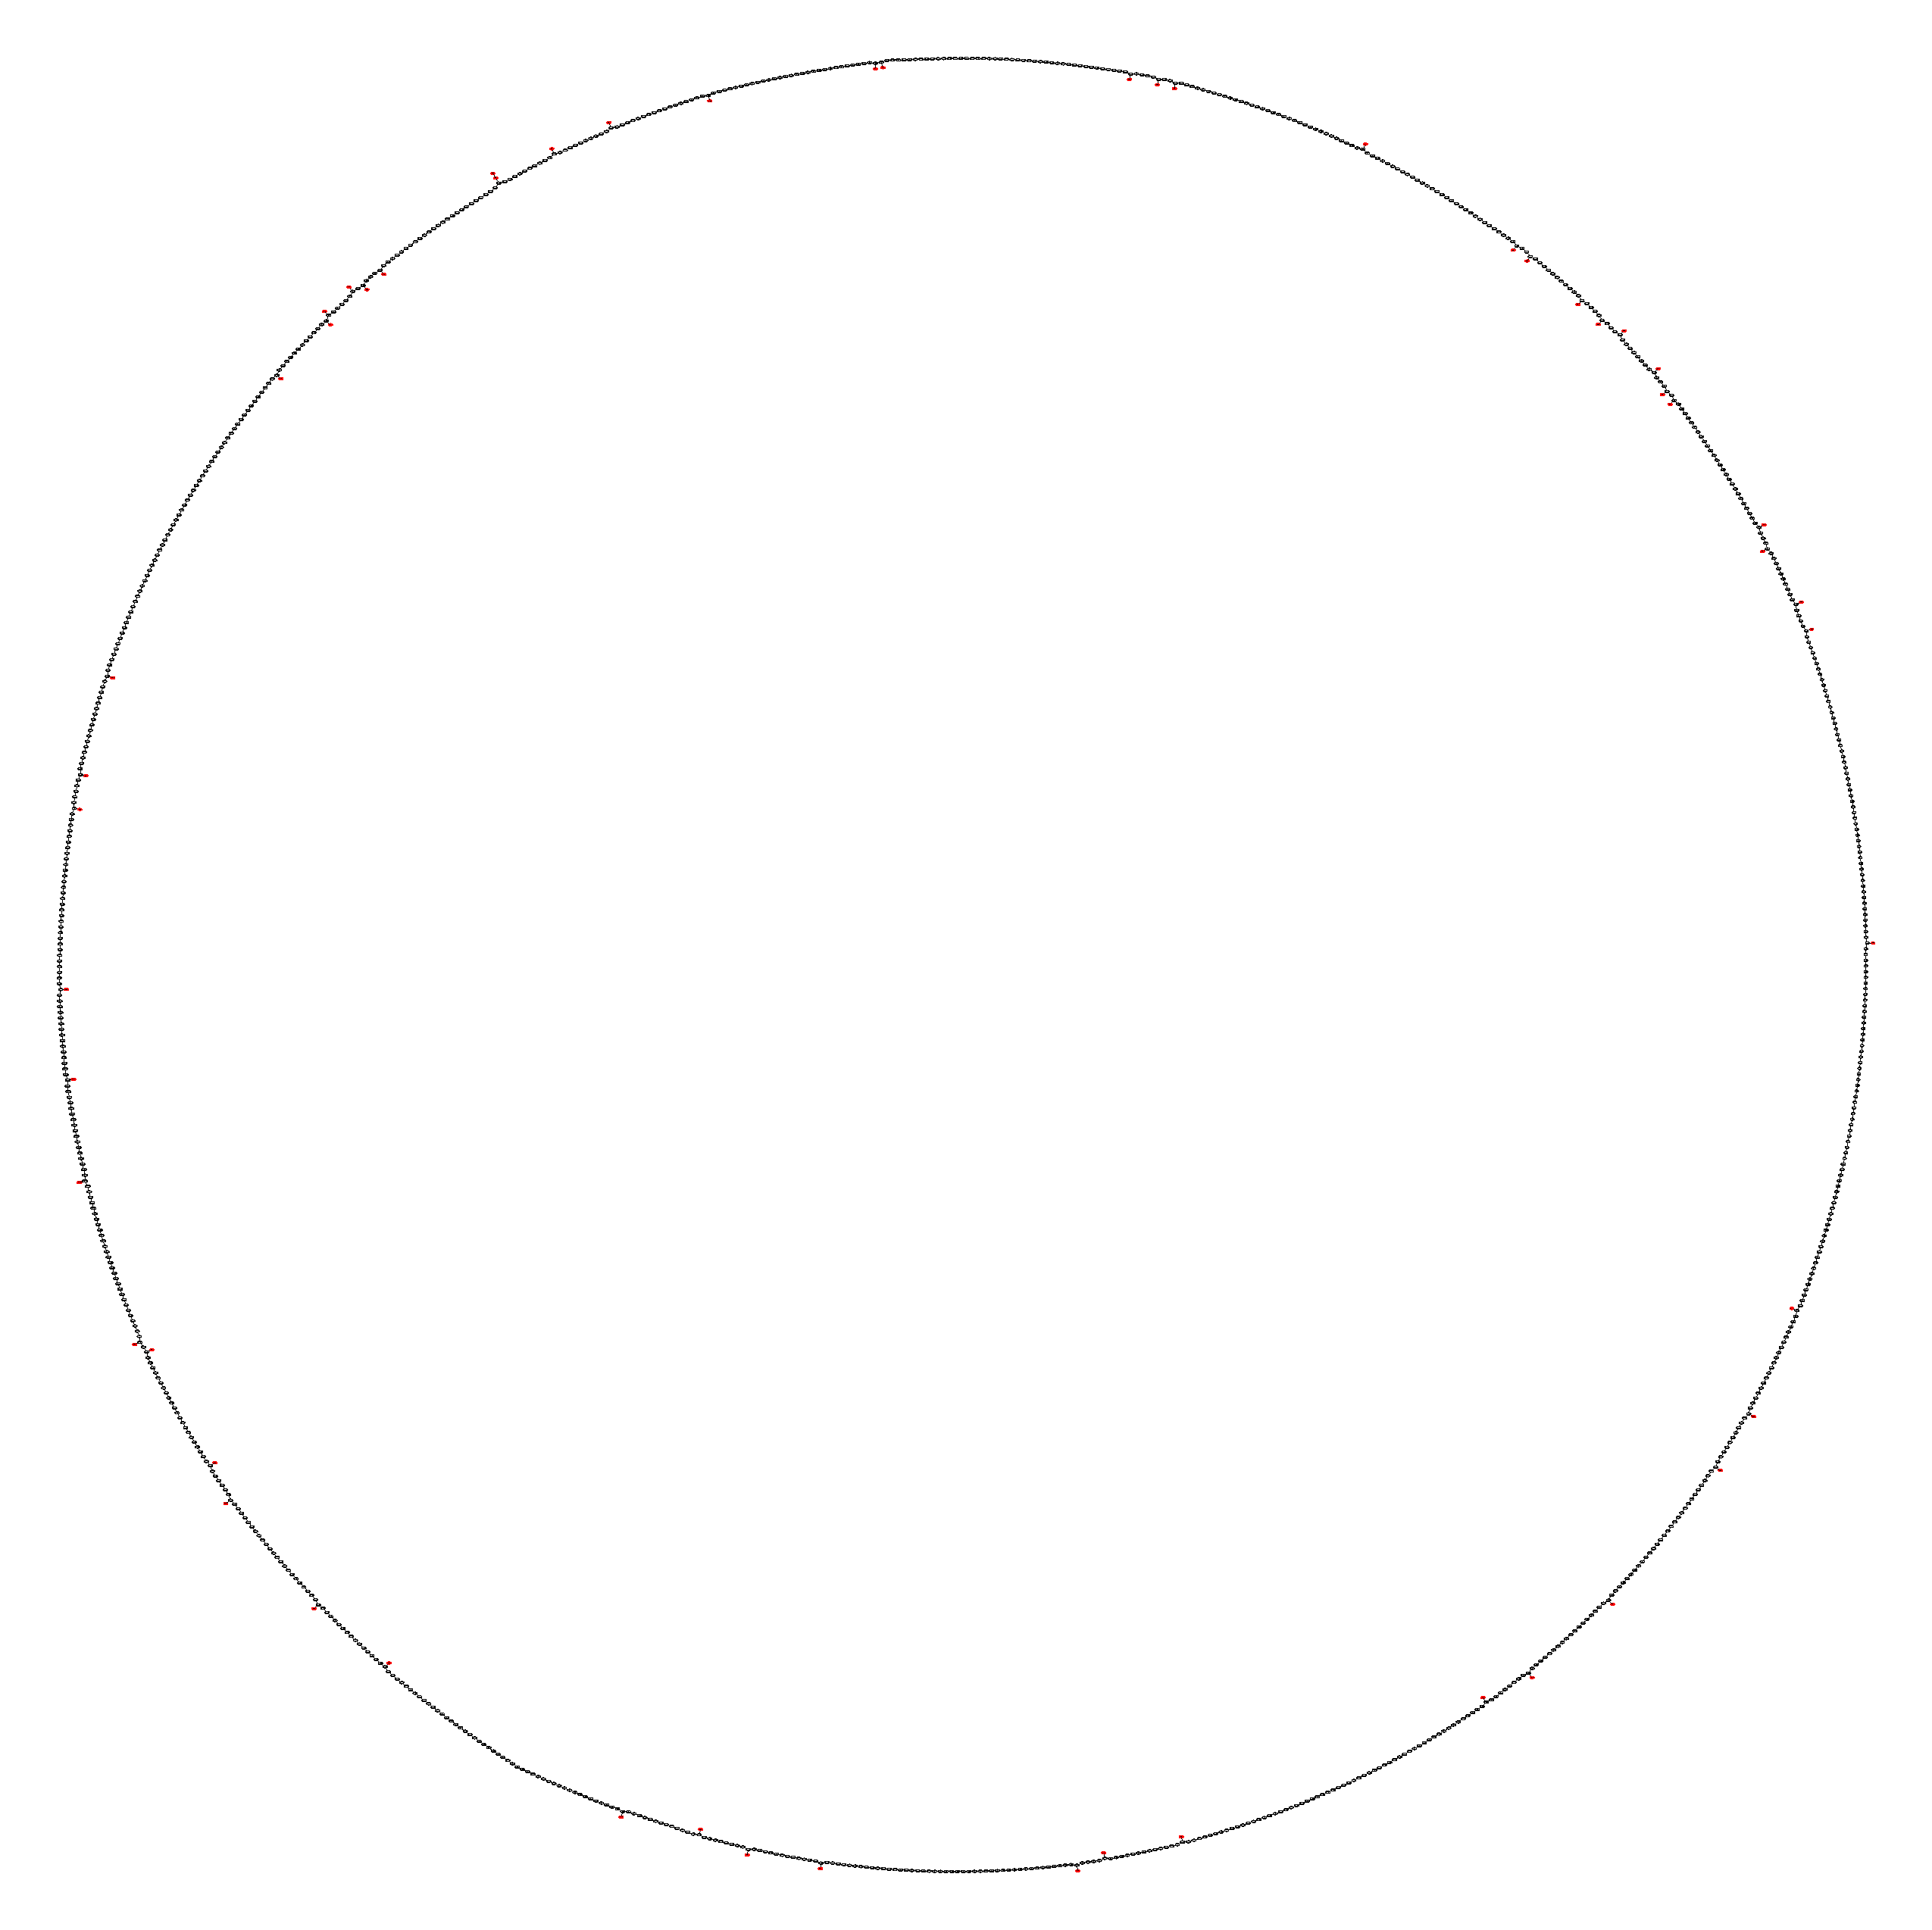
\includegraphics[width=2in]{f3b001}
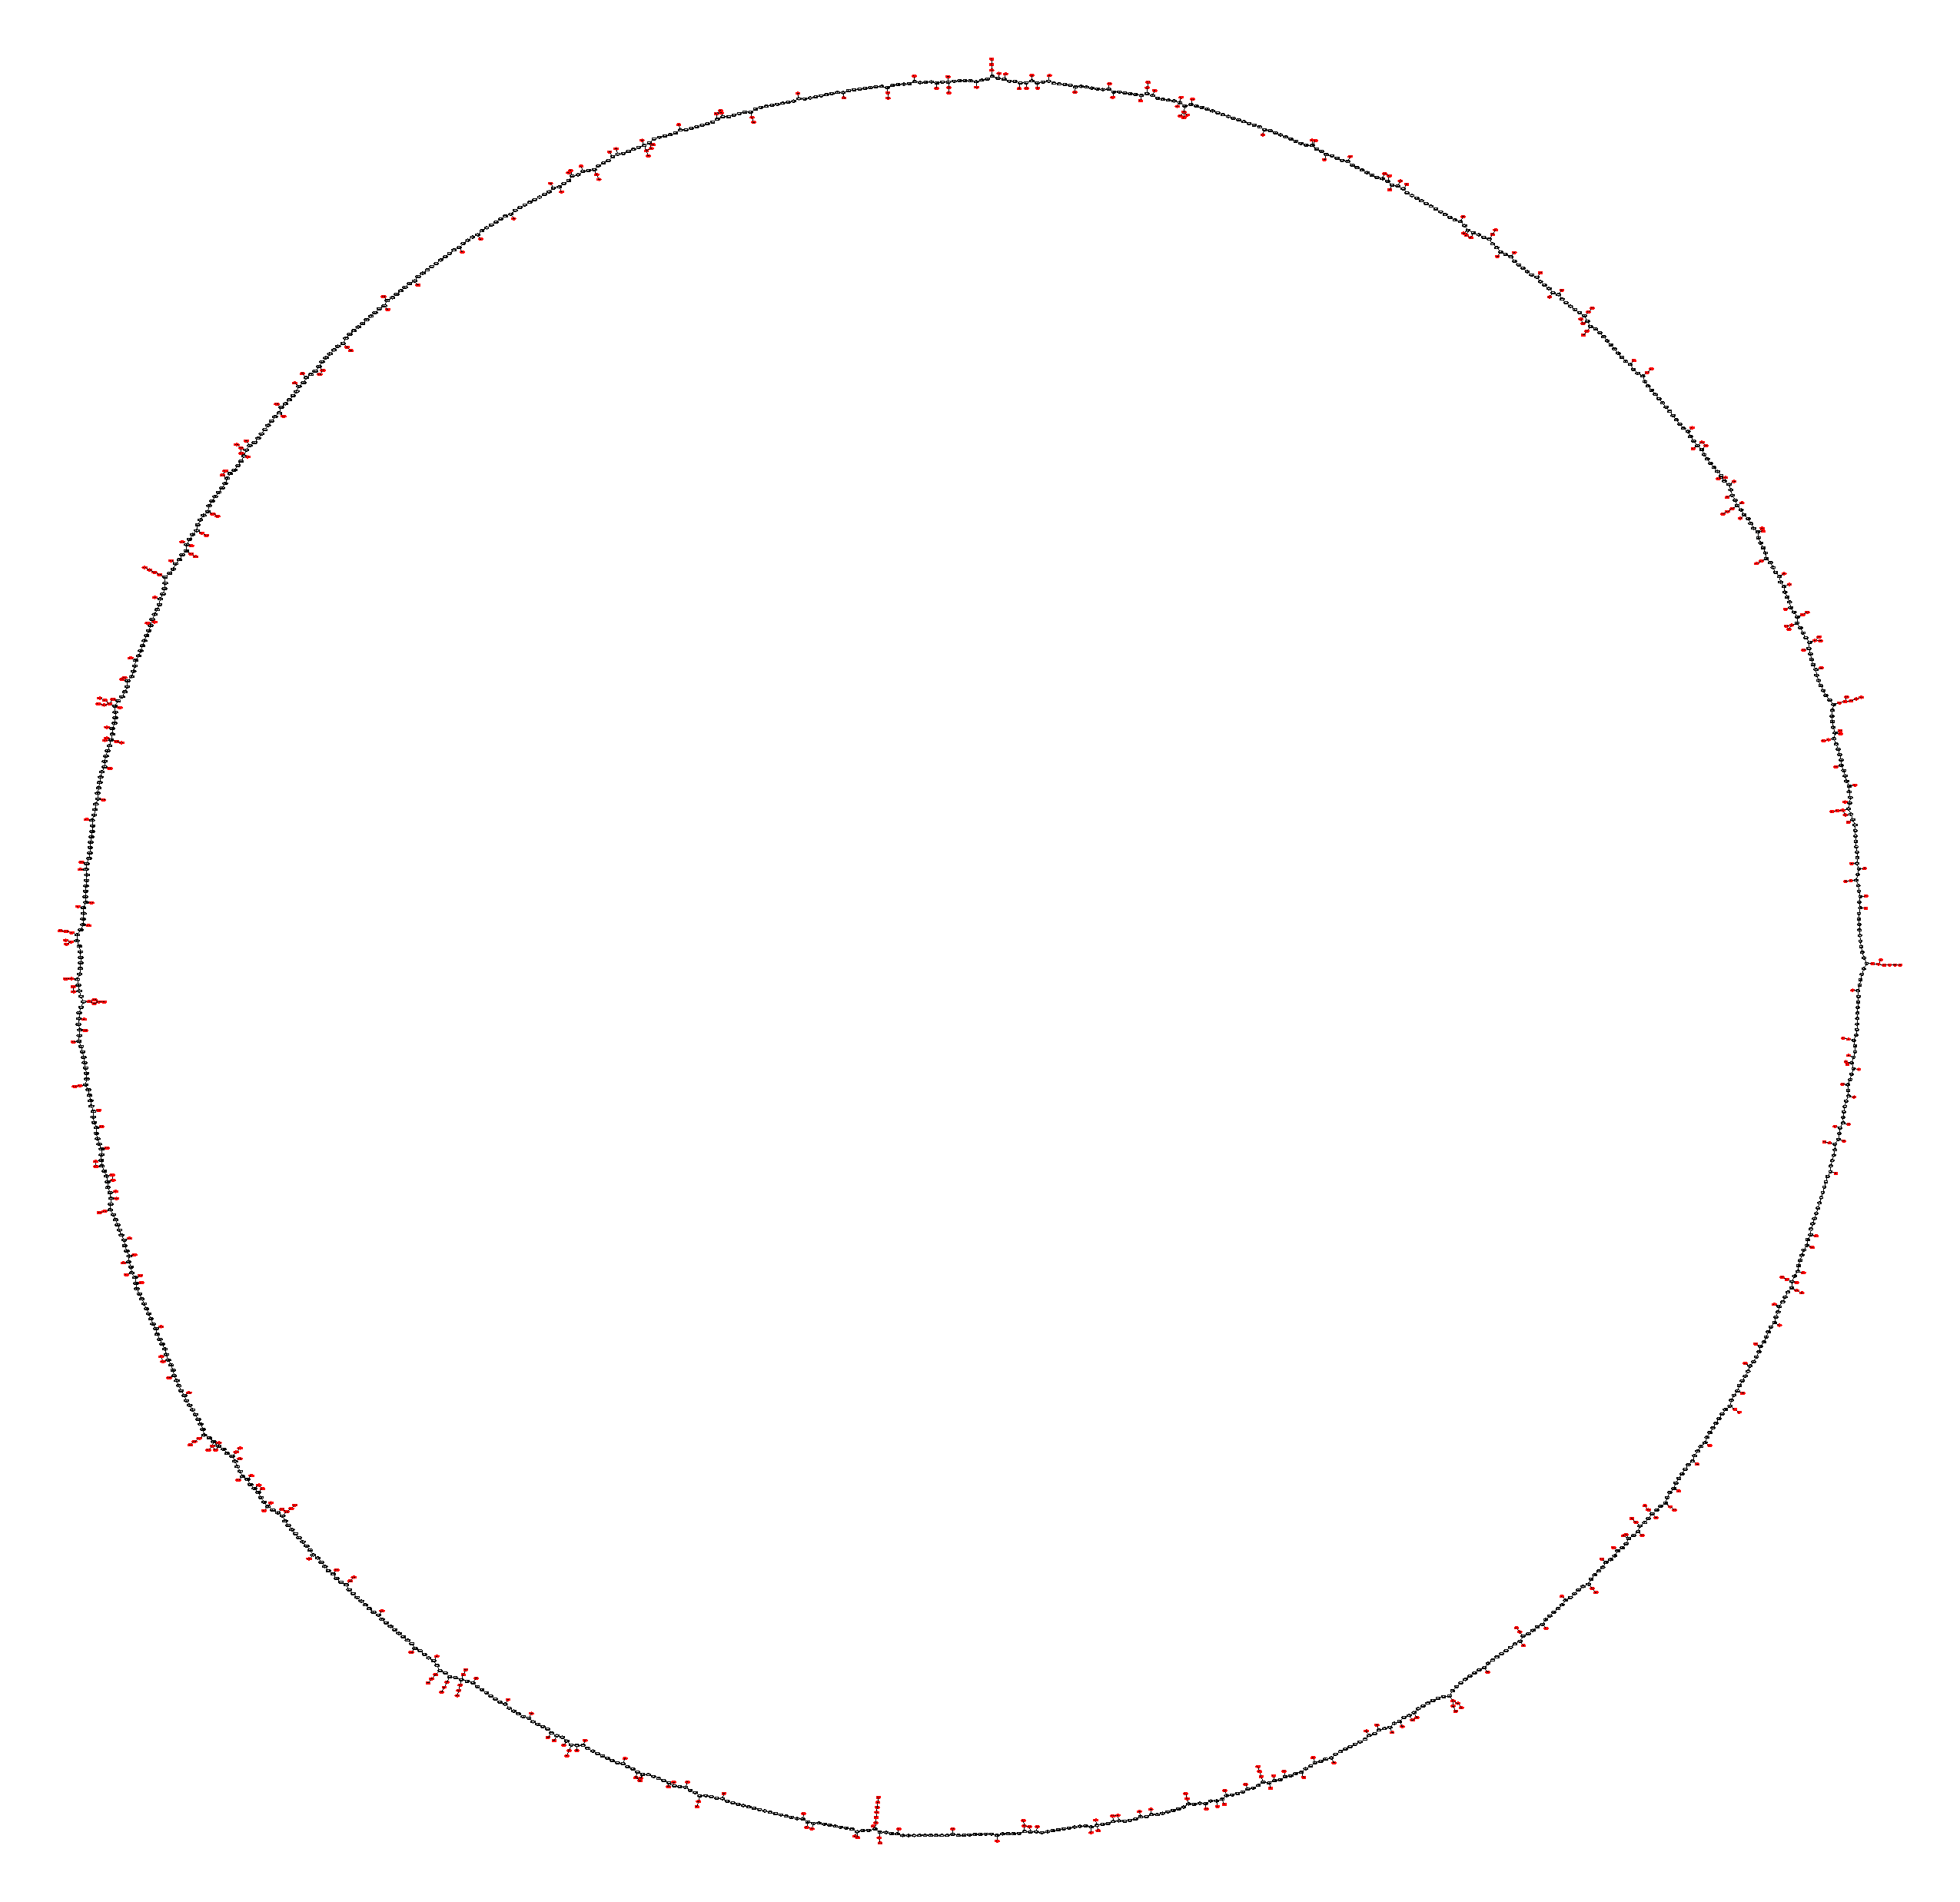
\includegraphics[width=2in]{f3b005}
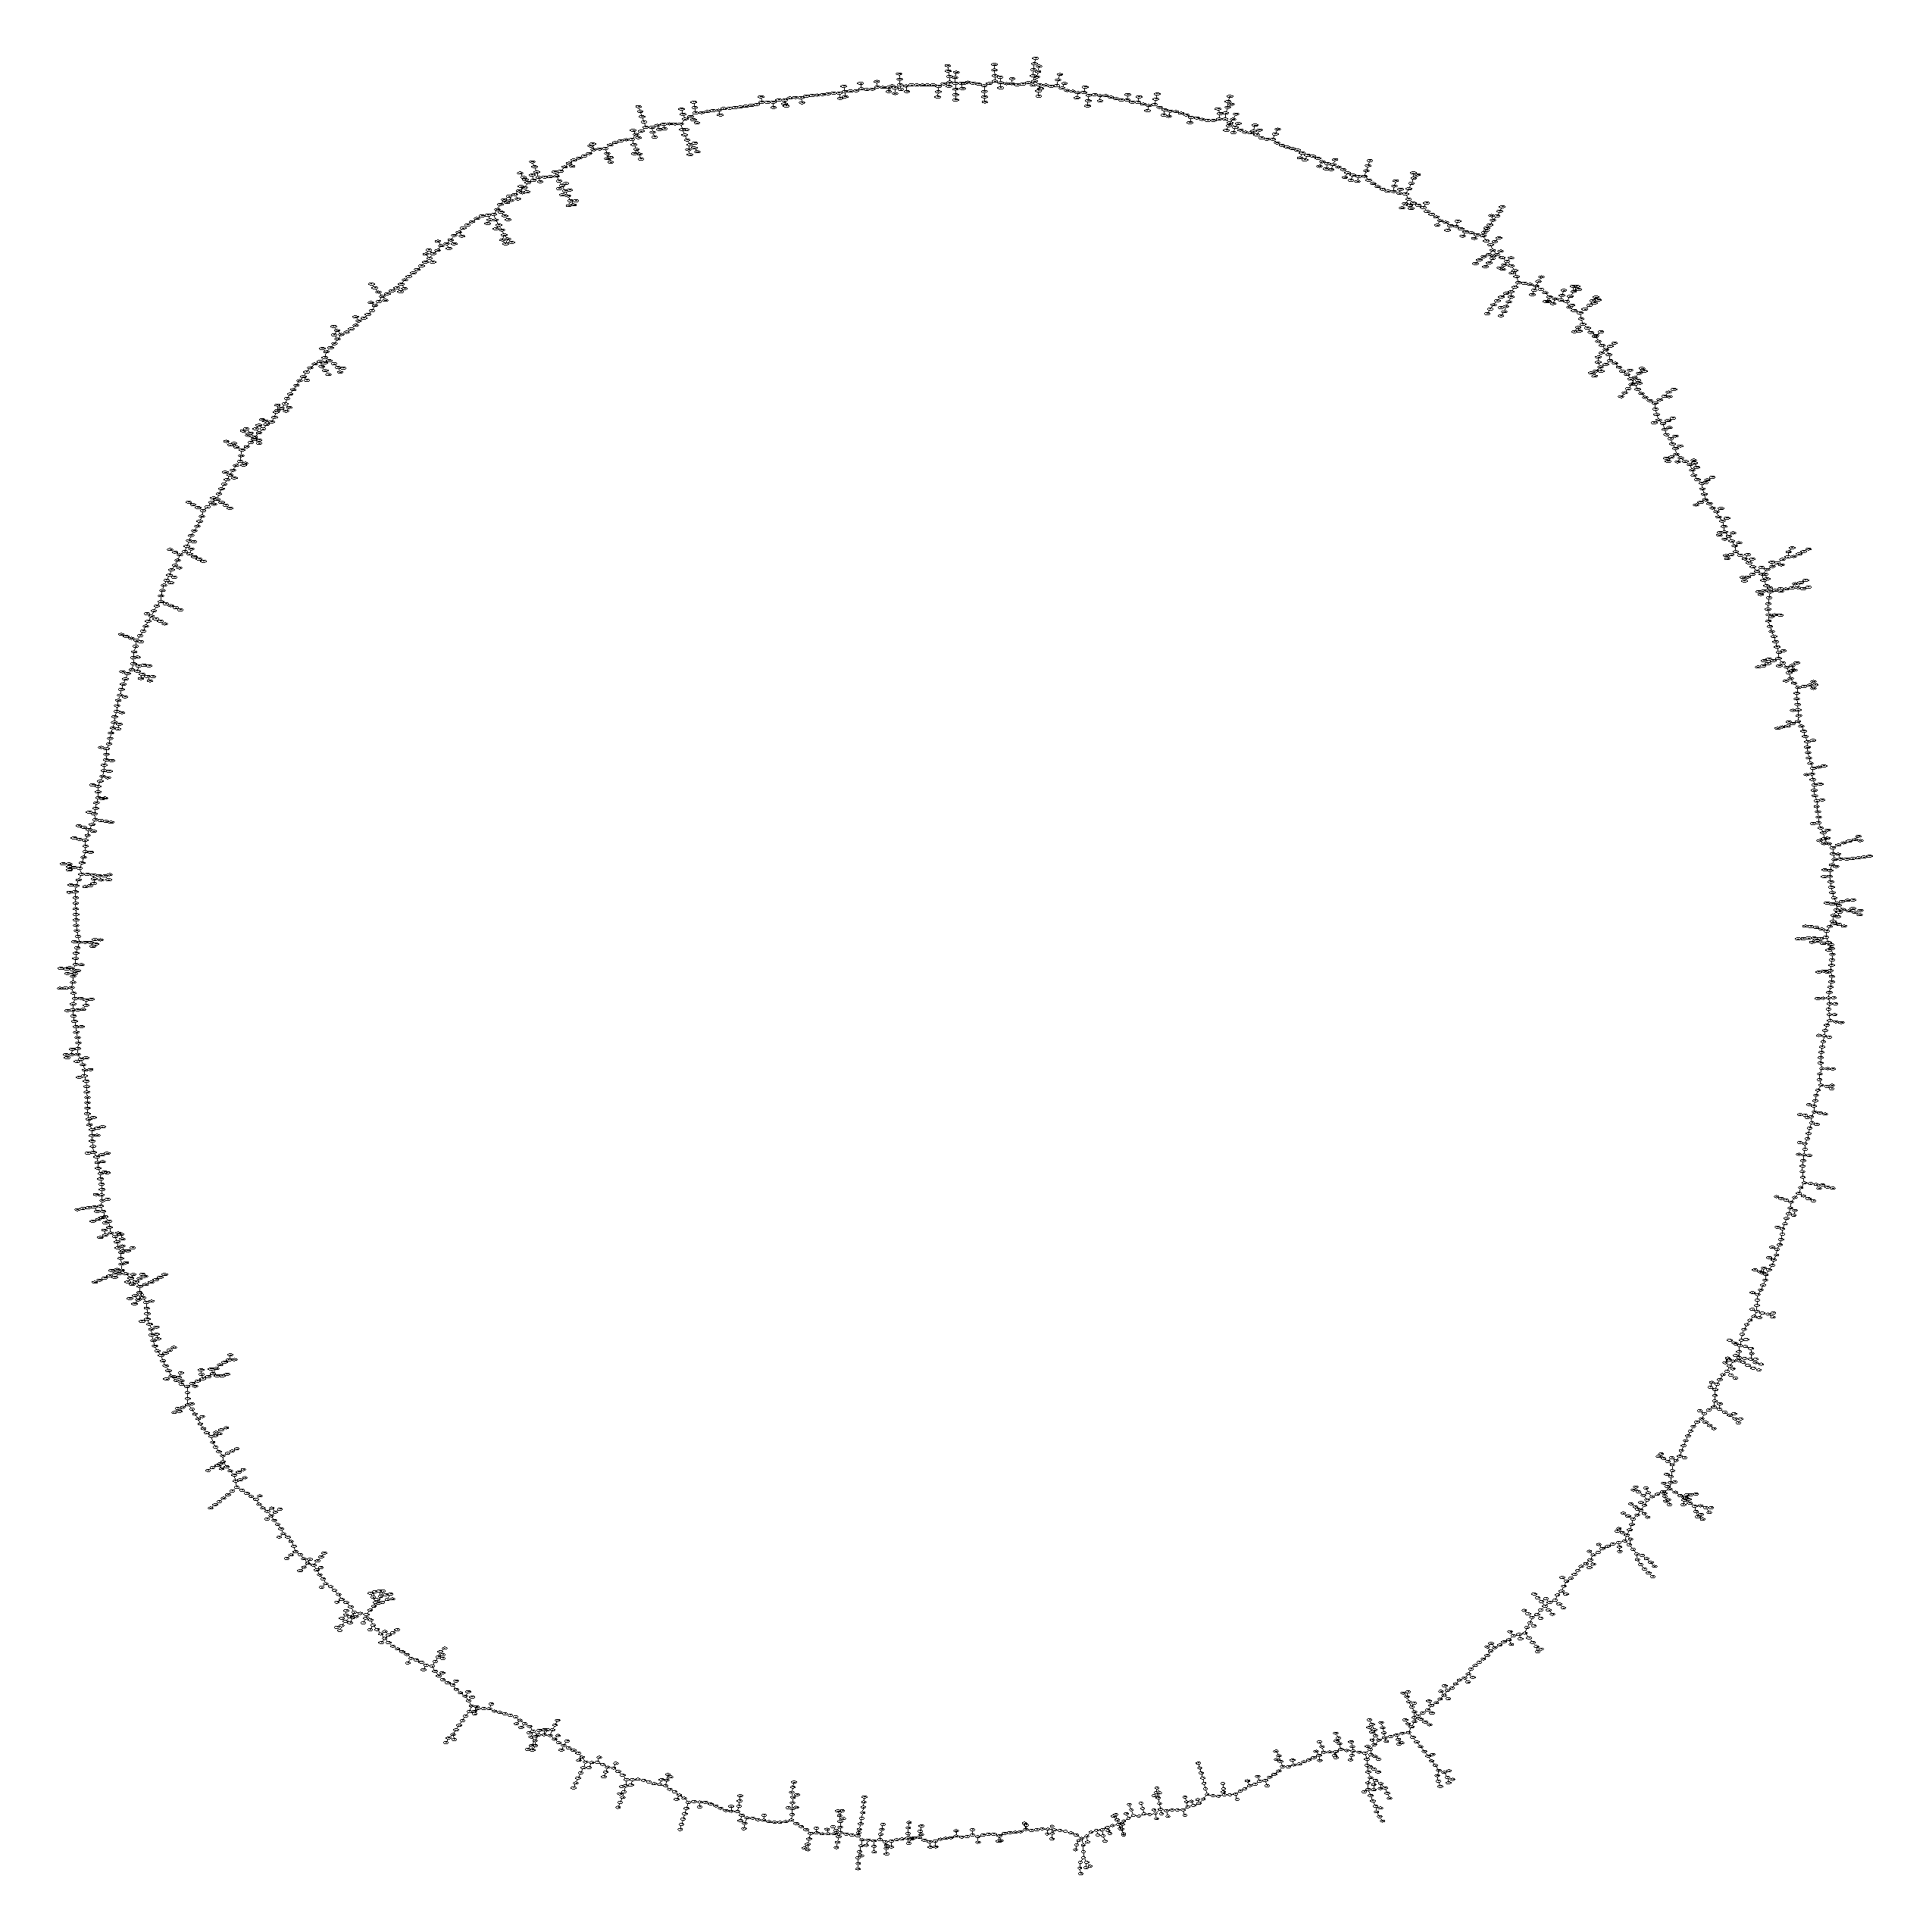
\includegraphics[width=2in]{f3b010}
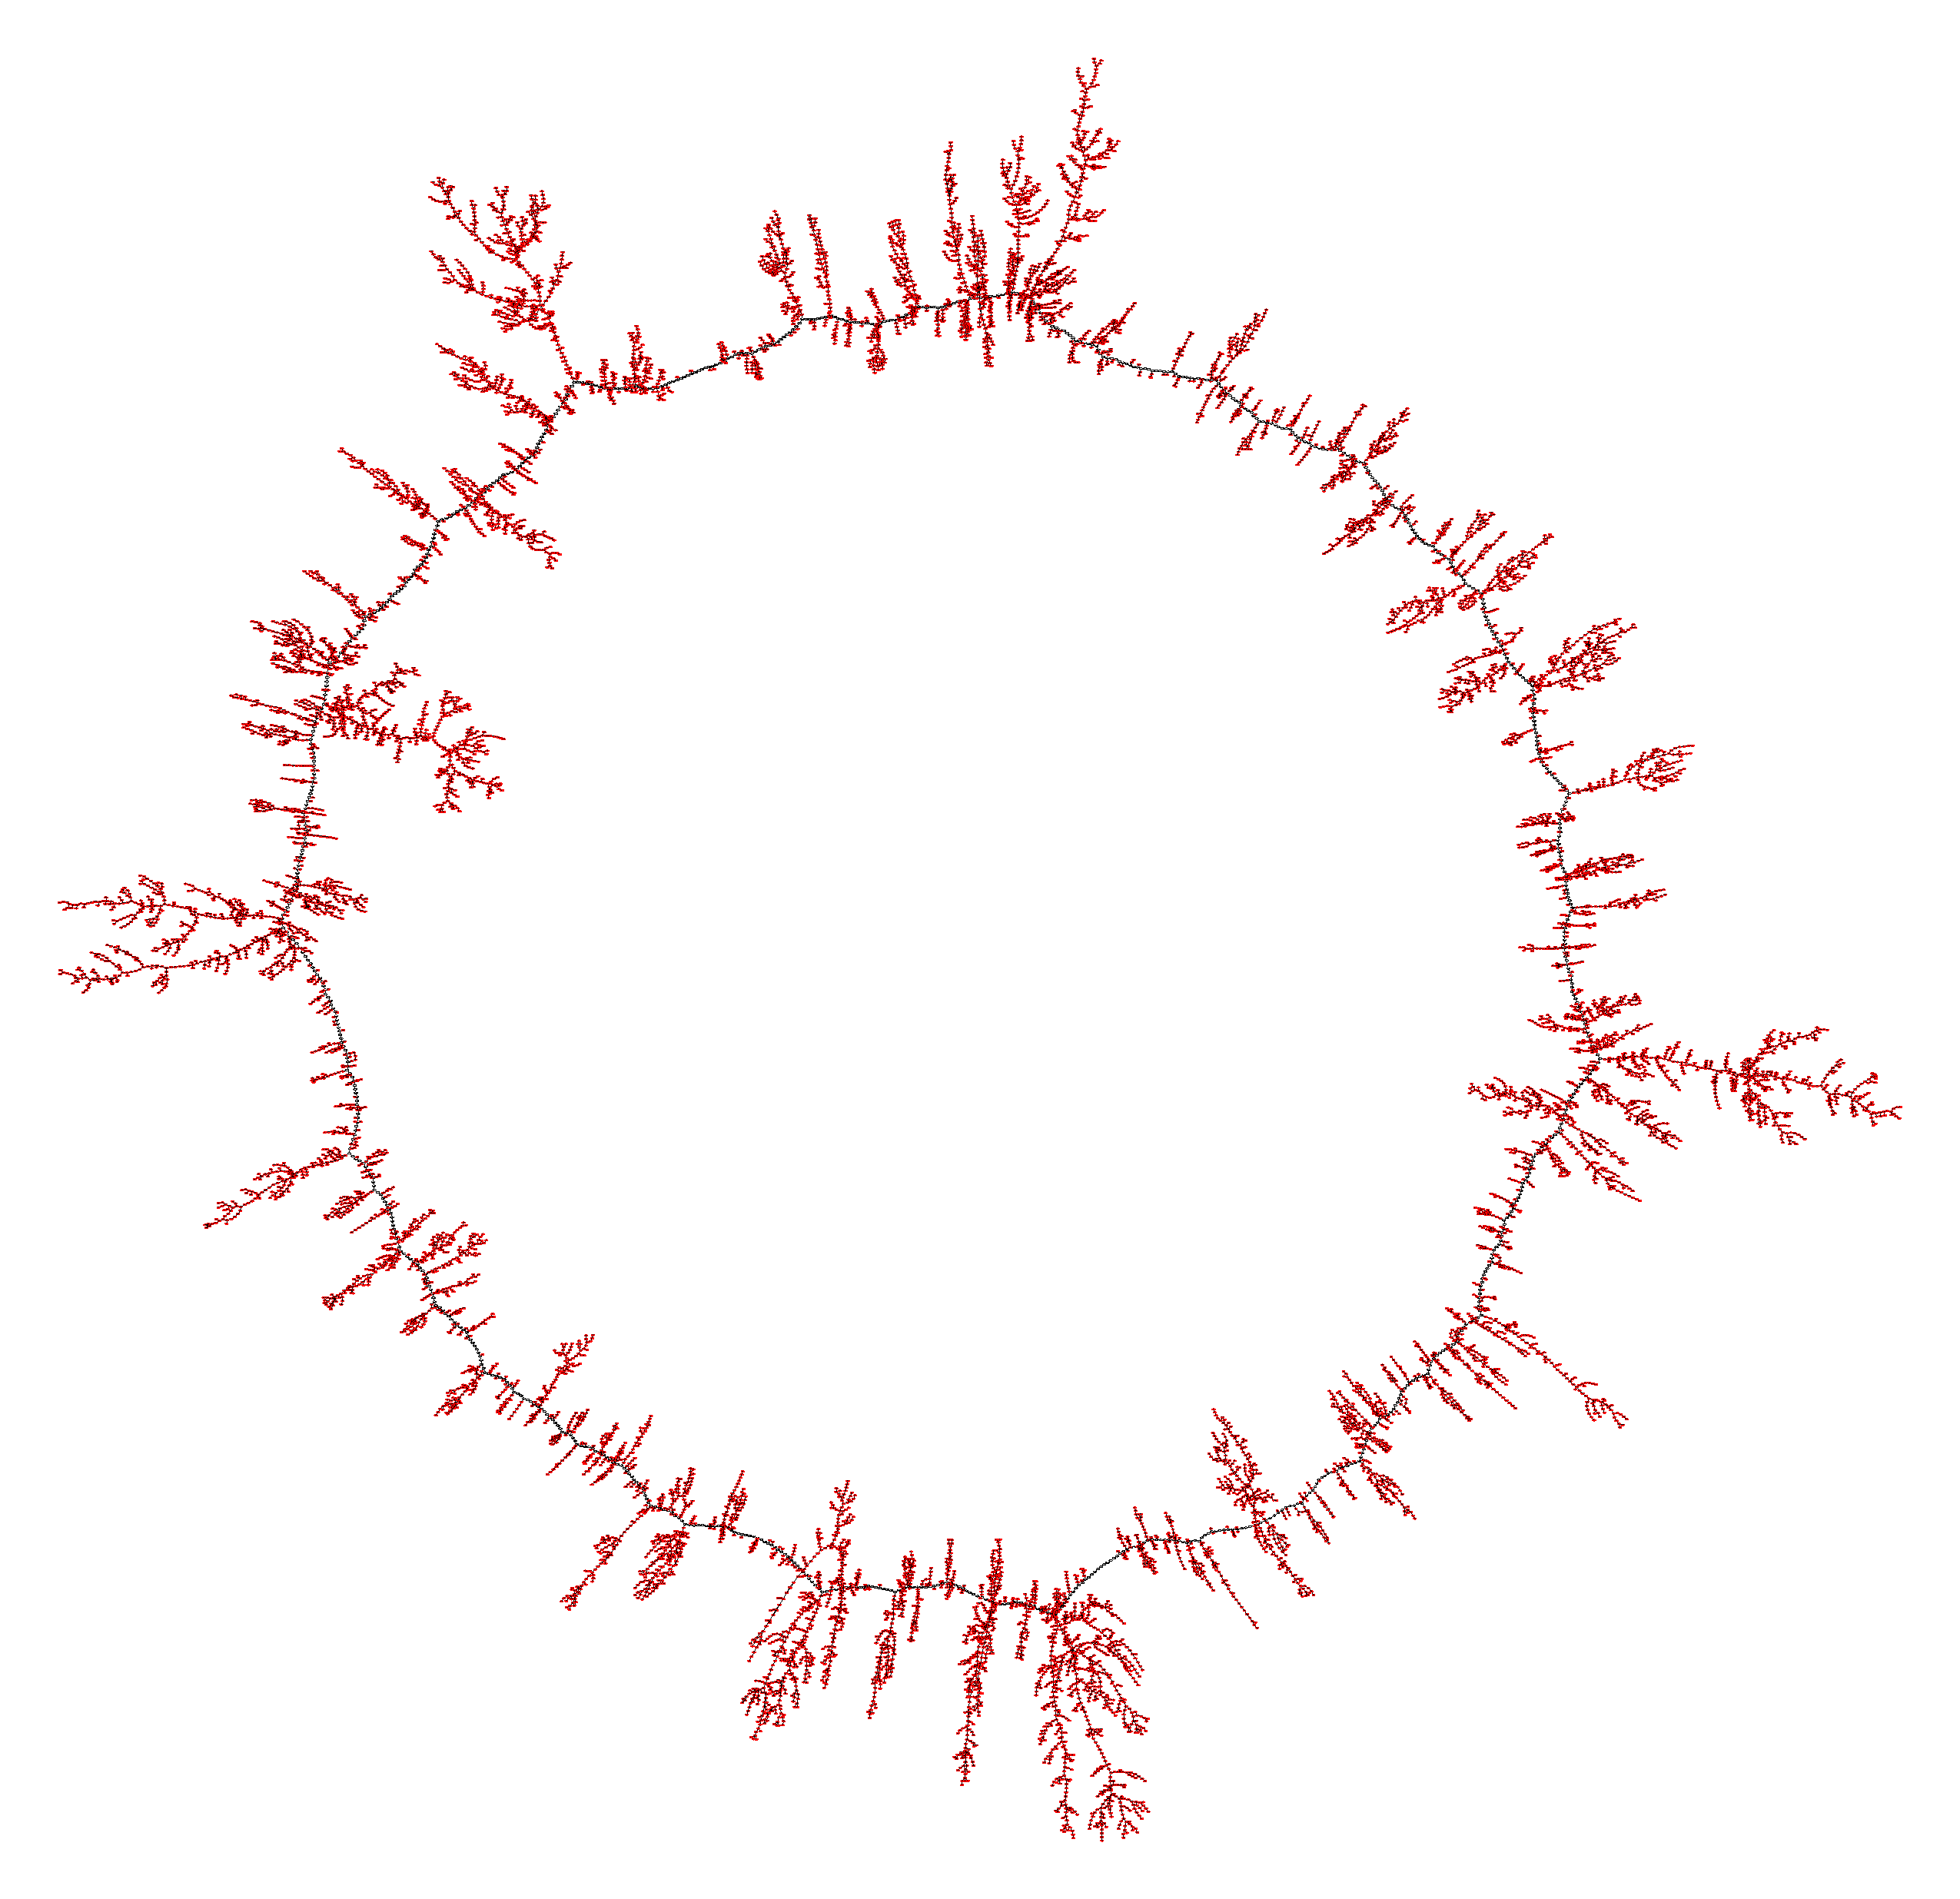
\includegraphics[width=2in]{f3b015}

\caption{Graph visualizations demonstrating the decreasing fidelity of
  graph structure with increasing false positive rate. Erroneous k-mers are 
  colored red and k-mers corresponding to the original generated sequence 
  are black. From top left
  to bottom right, the false positive rates are 0.01, 0.05, 0.10, and
  0.15.  Shortcuts ``across'' the graph are not created.}

\label{fig:circles}
\end{figure}

\begin{figure}
\center{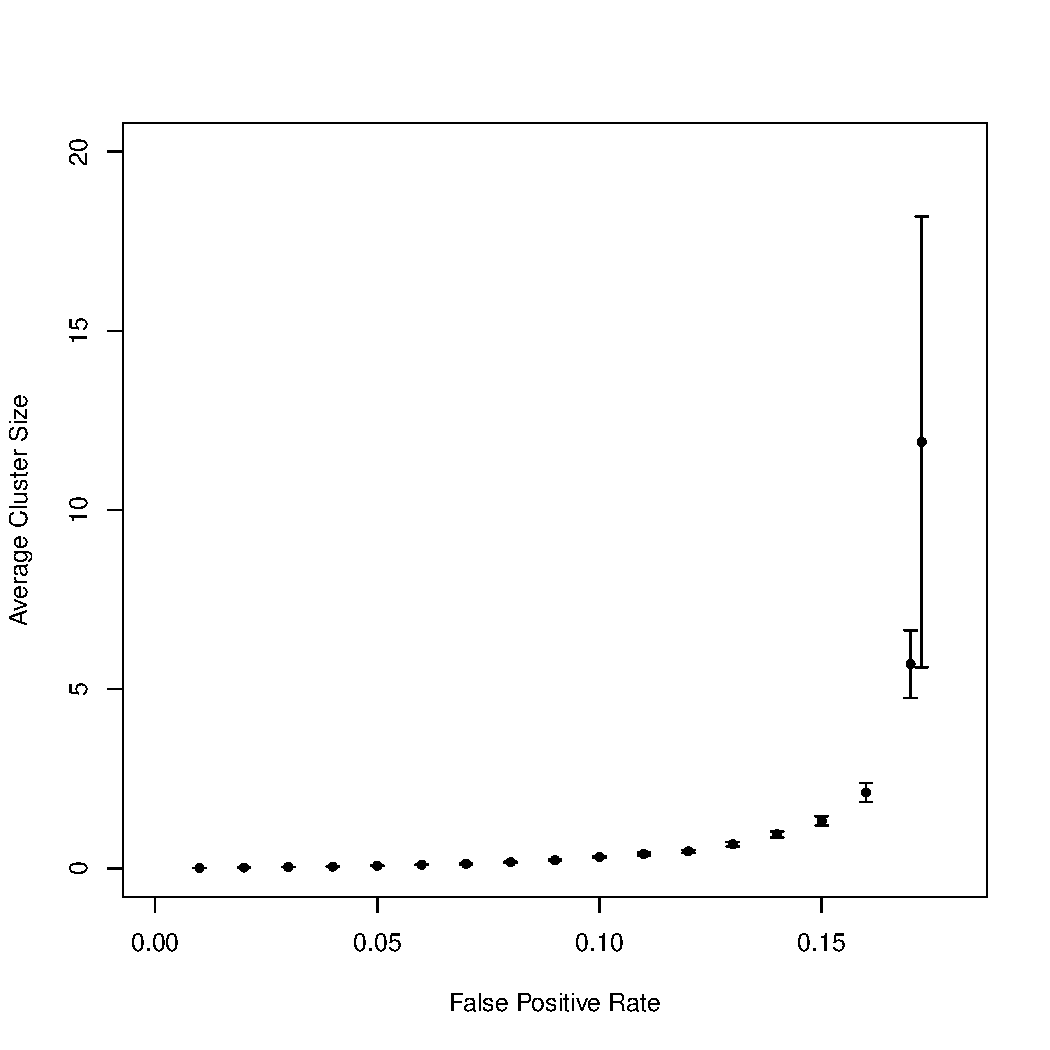
\includegraphics[width=5in]{newclust}}
\caption{Average component size versus false positive rate. The average 
component size sharply increases as the false positive 
rate approaches the percolation threshold.
}
\label{fig:clustersize}
\end{figure}

\begin{figure}
\center{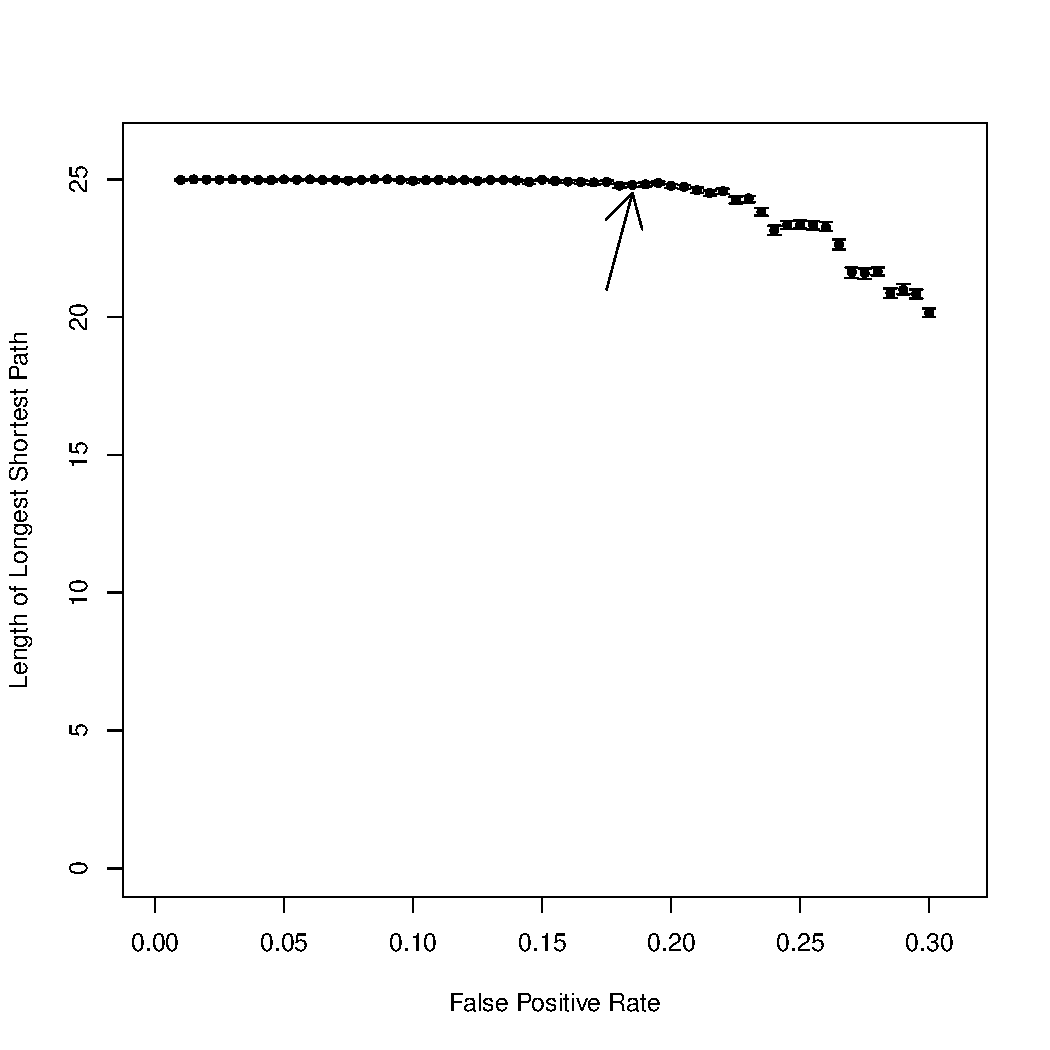
\includegraphics[width=5in]{newdiam}}

\caption{The diameter of randomly generated 58bp long circular
  chromosomes in 8-mer (i.e. a cycle of 50 8-mers) space remains 
constant for false
  positive rates up through 18.3\%. Only real (non-error) k-mers are considered for
  starting and ending points.}
\label{fig:diam}
\end{figure}

\begin{figure}
\center{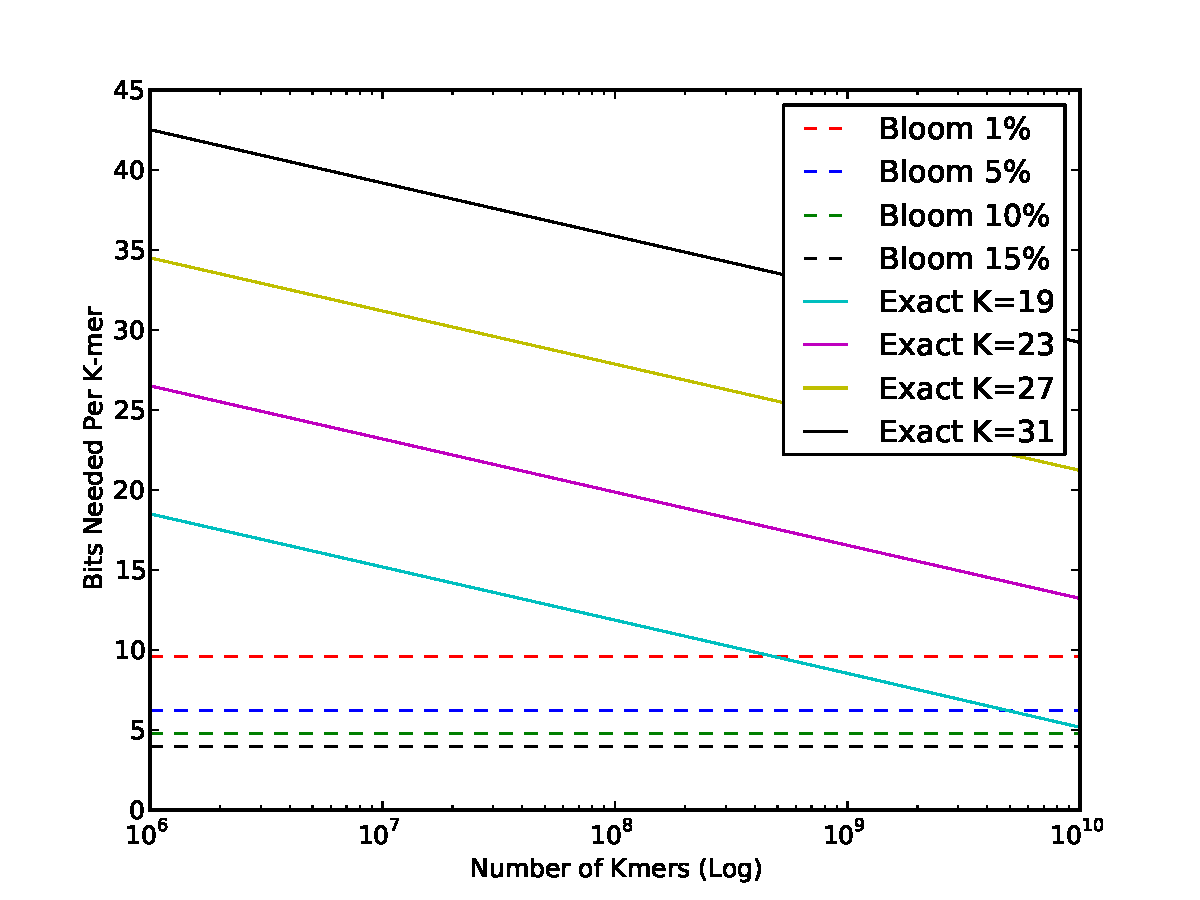
\includegraphics[width=6in]{memusg}}

\caption{Comparison between Bloom filters at different false positive 
rates with the information-theoretic lossless lower bound at different 
k values. Bloom filters are k independent and are more efficient than 
any lossless data structure for higher k due to greater sparseness in 
k-mers inserted compared to all possible k-mers.}

\label{fig:membound}
\end{figure}

% Memory
%  use is maximum memory required in gigabytes during partitioning,
%  with the given improvement ratio over using the ABySS assembler on
%  the unpartitioned data, which required 33 GB.  N partitions is the
%  total number of partitions containing more than 500 k-mers, and D is
%  the largest partition size in reads.}

\begin{table*}
\centering
\caption{Bits per k-mer for various false positive rates.}
\begin{tabular*}{\hsize}{@{\extracolsep{\fill}}cccc}
\hline
False positive rate & Bits/k-mer \\ \hline
0.1 \% & 14.35 \cr
1 \% & 9.54 \cr
5 \% & 6.22 \cr
10 \% & 4.78 \cr
15 \% & 3.94 \cr
20 \% & 3.34 \cr
\hline\end{tabular*}
\label{table:bitskmer}
\end{table*}

\begin{table}
\centering

\caption{Effects of loading \emph{E. coli} data at different false positive rates}
\begin{tabular*}{\hsize}{@{\extracolsep{\fill}}ccccccc}
\hline
Graph & Total k-mers & False connected k-mers & \% Real & Deg $> 2$ & Mem (bytes) \\ \hline
\emph{E. coli} at 0\% & 4,530,123 & 0 & 100 & 50,605 & $2.1 \times 10^{9}$ \\
\emph{E. coli} at 1\% & 4,814,050 & 283,927 & 94.1 & 313,844 & $5.4 \times 10^6$ \\
\emph{E. coli} at 5\% & 6,349,301 & 1,819,178 & 71.3 & 1,339,102 & $3.5 \times 10^6$ \\
\emph{E. coli} at 15\% & 31,109,523 & 26,579,400 & 14.6 & 10,522,482 & $2.2 \times 10^6$ \\
Reads at 0\% & 45,566,033 & 41,036,029 & 9.9 & 7,699,309 & $2.1 \times 10^{9}$ \\
Reads at 1\% & 48,182,271 & 43,652,265 & 9.4 & 31,600,208 & $5.4 \times 10^7$ \\
Reads at 5\% & 62,019,545 & 57,489,537 & 7.3 & 42,642,203 & $3.6 \times 10^7$ \\
Reads at 15\% & 231,687,063 & 227,157,037 & 1.9 & 113,489,902 & $2.3 \times 10^7$ \\
\hline
\end{tabular*}
\label{table:ecoli}
\end{table}

\begin{table*}
\centering
\caption{Partitioning results on a soil metagenome at k=31.}

\begin{tabular*}{\hsize}{@{\extracolsep{\fill}}cccc}
False positive rate & Total memory use (improvement) & Largest partition size in reads \cr
\hline
1\% & 1.75GB (18.8x) & 344,426 \cr
5\% & 1.20GB (27.5x) & 344,426 \cr
10\% & 0.96GB (34.37x) & 344,426 \cr
15\% & 0.83GB (39.75x) & 344,426 \cr
\hline
\end{tabular*}

\label{table:parts}
\end{table*}

\setcounter{figure}{0}
\makeatletter
\renewcommand{\thefigure}{S\@arabic\c@figure}
\begin{figure}
\center{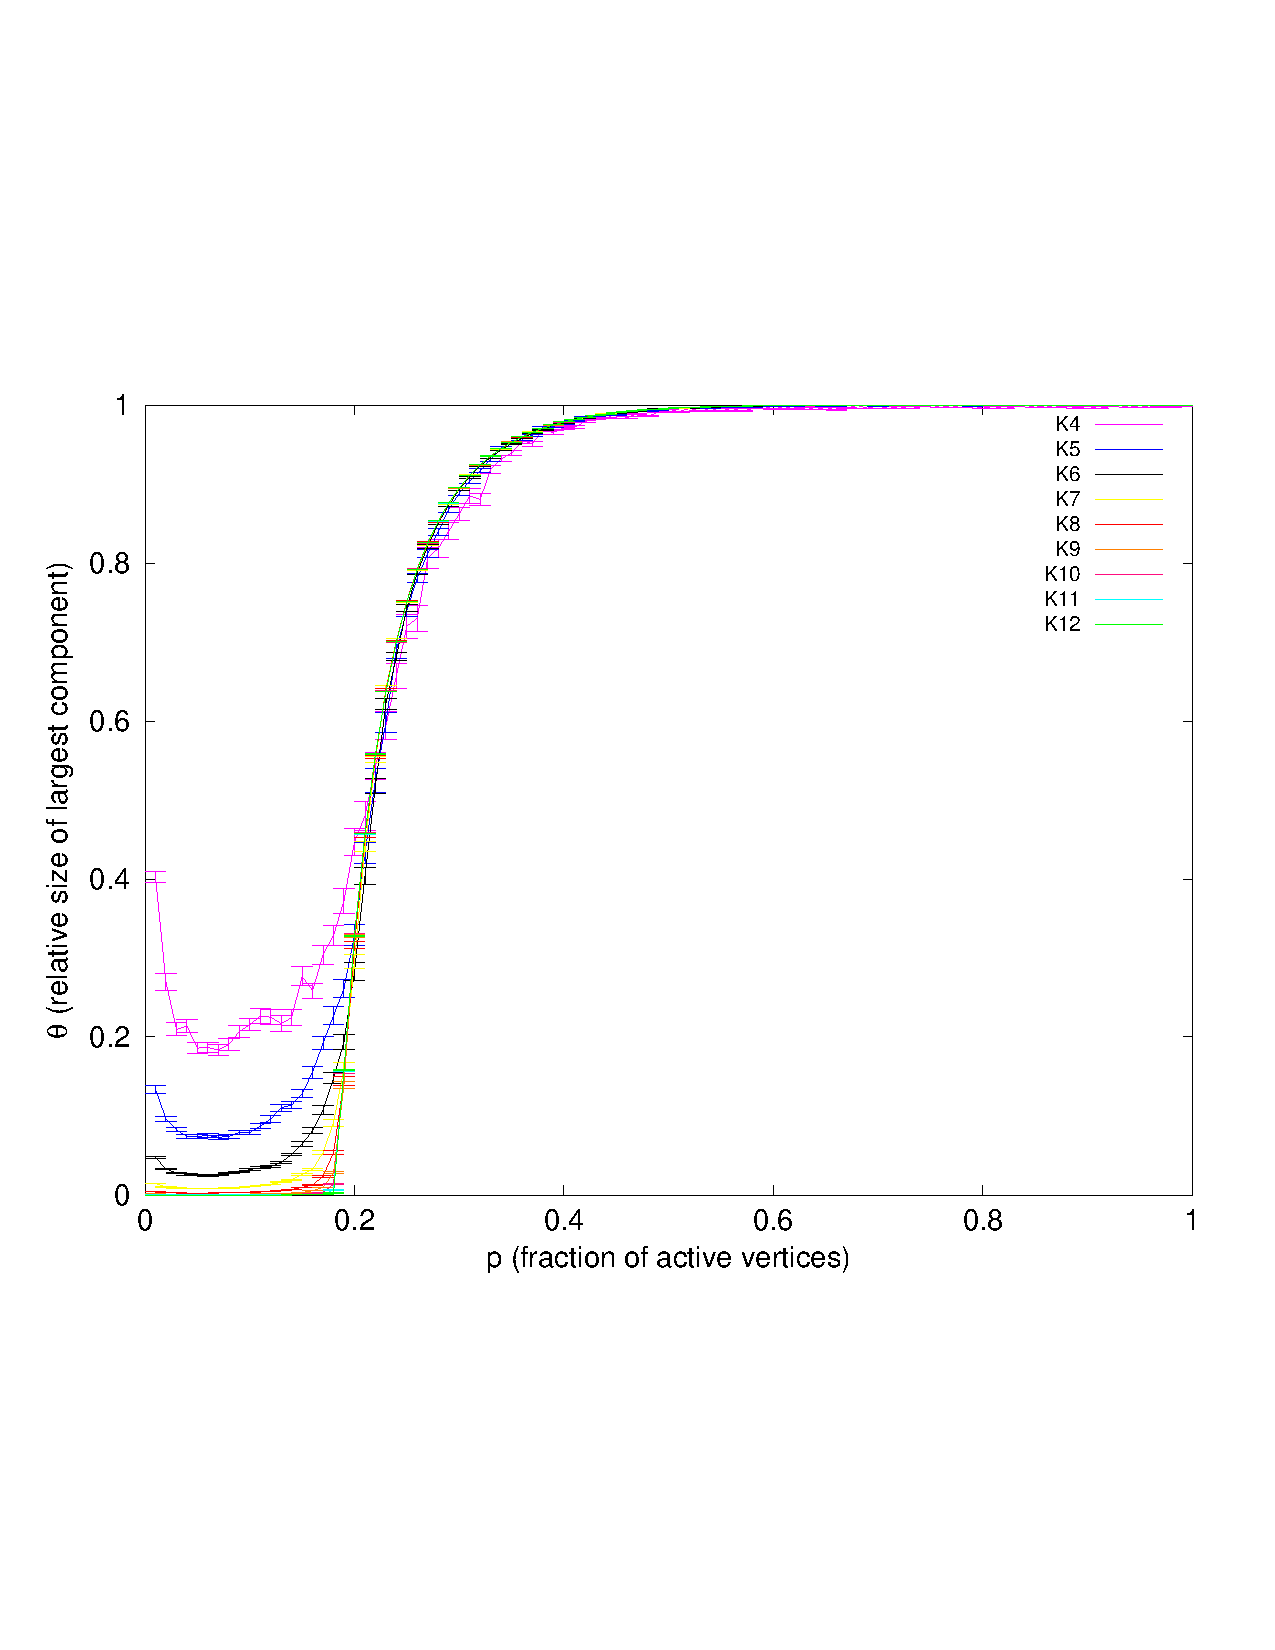
\includegraphics[width=5in]{s1}}

\caption{Demonstration of k independence by determining the
  percolation threshold with multiple values of k (5-12).  $p$ on the
  x axis is the fraction of nodes present, and $\theta$ on the y axis
  is the fraction of nodes in the largest component.  Lower values of
  k have greater finite size sampling errors.}

\label{fig:kindependence}
\end{figure}

\begin{figure}
\center{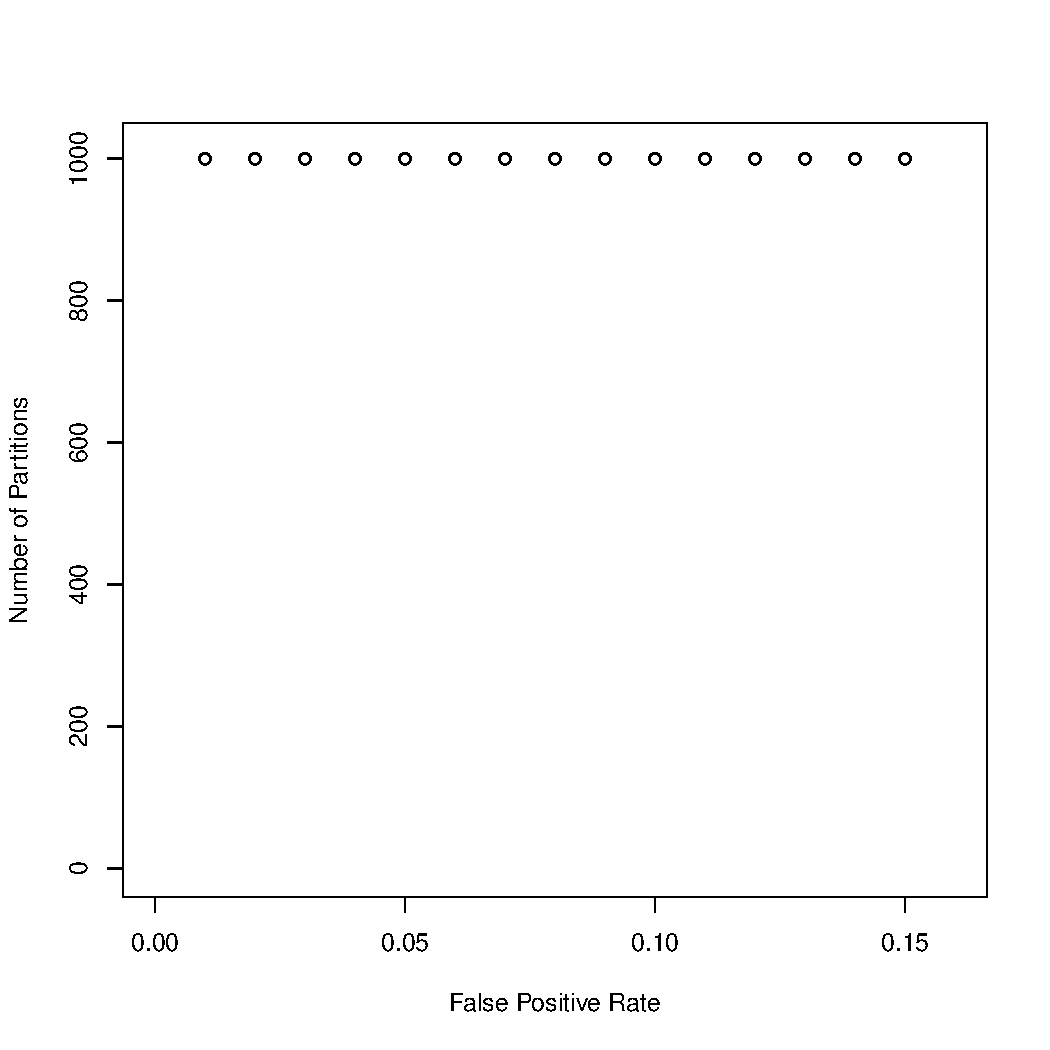
\includegraphics[width=5in]{newpart}}

\caption{The graph shows the number of partitions for a simulated dataset with
  1,000 contigs of 10,000 bp each (circles). For $n=5$ different
  combinations of hash table sizes, there was no variation in results
  for the simulated dataset.}

\label{fig:partfp}
\end{figure}

\makeatother

%% @@effects of local graph elaboration on partitioning/traversal alg?
%% @@graphsize filtering vs partitioning?
%% @@change mem/bits to mem/bytes.
%% @@go back and refer to tables and figures in discussion, too.

\end{document}
